\documentclass[11pt]{article}
\pdftrailerid{}
\pdfinfoomitdate=1
\pdfinfo{/CreationDate (D:20260924000000Z) /ModDate (D:20260924000000Z)}
\usepackage[T1]{fontenc}
\usepackage[utf8]{inputenc}
\usepackage{lmodern}
\usepackage{amsmath,amssymb,amsthm,mathtools}
\usepackage[letterpaper,margin=1.08in]{geometry}
\usepackage{microtype}
\usepackage{enumitem}
\usepackage{booktabs,array,tabularx}
\usepackage{xcolor}
\usepackage{tikz}
\usetikzlibrary{arrows.meta,positioning,calc}
\usepackage{hyperref}
\usepackage{bookmark}
\input{glyphtounicode}
\pdfglyphtounicode{mu}{03BC}
\pdfglyphtounicode{Delta}{0394}
\pdfglyphtounicode{backslash}{2216}
\pdfglyphtounicode{mapsto}{007C}
\pdfglyphtounicode{parenleftbig}{0028}
\pdfglyphtounicode{parenrightbig}{0029}
\pdfglyphtounicode{braceleftbig}{007B}
\pdfglyphtounicode{bracerightbig}{007D}
\pdfglyphtounicode{parenleftbigg}{0028}
\pdfglyphtounicode{parenrightbigg}{0029}
\pdfglyphtounicode{braceleftbigg}{007B}
\pdfglyphtounicode{bracerightbigg}{007D}
\pdfglyphtounicode{parenleftBigg}{0028}
\pdfglyphtounicode{parenrightBigg}{0029}
\pdfglyphtounicode{braceleftBigg}{007B}
\pdfglyphtounicode{bracerightBigg}{007D}
\pdfglyphtounicode{vextendsingle}{23D0}
\pdfglyphtounicode{vextenddouble}{2016}
\pdfglyphtounicode{summationtext}{2211}
\pdfglyphtounicode{summationdisplay}{2211}
\pdfglyphtounicode{producttext}{220F}
\pdfglyphtounicode{productdisplay}{220F}
\pdfglyphtounicode{integraldisplay}{222B}
\pdfglyphtounicode{radicalbig}{221A}
\pdfglyphtounicode{radicalBig}{221A}
\pdfglyphtounicode{radicalbigg}{221A}
\pdfgentounicode=1
\hypersetup{
  colorlinks=true,
  linkcolor=blue!45!black,
  citecolor=blue!45!black,
  urlcolor=blue!45!black,
  pdftitle={Additive hardness and unbounded configuration gaps in bin packing},
  pdfauthor={OpenAI},
  pdfsubject={Bin packing, additive approximation, configuration linear programming, and the Modified Integer Round-Up Conjecture},
  pdfcreator={pdfLaTeX},
  bookmarksnumbered=true,
  pdfdisplaydoctitle=true
}
\newcommand{\R}{\mathbb R}
\newcommand{\N}{\mathbb N}
\newcommand{\Z}{\mathbb Z}
\newcommand{\Q}{\mathbb Q}
\newcommand{\classP}{\mathsf P}
\newcommand{\classNP}{\mathsf{NP}}
\newcommand{\OPT}{\operatorname{OPT}}
\newcommand{\LP}{\operatorname{OPT}_{\mathrm{LP}}}
\newcommand{\len}{\operatorname{len}}
\newcommand{\ind}{\mathbf{1}}
\newcommand{\Tp}{\mathrm{T}_{+}}
\newcommand{\Tm}{\mathrm{T}_{-}}
\newcommand{\Srow}{\mathrm{S}}
\newcommand{\Zanc}{\mathrm{Z}}
\newcommand{\Yanc}{\mathrm{Y}}
\newcommand{\Up}{\mathrm{U}_{+}}
\newcommand{\Um}{\mathrm{U}_{-}}
\newcommand{\Waux}{\mathrm{W}}
\newcommand{\DM}{\mathrm{D}_{\mathrm M}}
\newcommand{\DG}{\mathrm{D}_{\mathrm G}}
\newcommand{\FT}{\mathrm{F}_{\mathrm T}}
\newcommand{\FM}{\mathrm{F}_{\mathrm M}}
\newcommand{\FG}{\mathrm{F}_{\mathrm G}}
\newtheorem{theorem}{Theorem}[section]
\newtheorem{proposition}[theorem]{Proposition}
\newtheorem{lemma}[theorem]{Lemma}
\newtheorem{corollary}[theorem]{Corollary}
\theoremstyle{definition}
\newtheorem{definition}[theorem]{Definition}
\theoremstyle{remark}
\newtheorem{remark}[theorem]{Remark}
\numberwithin{equation}{section}
\setlist[enumerate]{itemsep=3pt,topsep=6pt}
\setlist[itemize]{itemsep=3pt,topsep=6pt}
\setlength{\emergencystretch}{1.5em}
\allowdisplaybreaks[1]
\widowpenalty=8000
\clubpenalty=8000
\makeatletter
\renewcommand{\@maketitle}{%
  \newpage
  \null
  \vskip 2em
  \begin{center}%
    {\LARGE \@title\par}%
    \vskip 0.8em
    {\large \@author\par}%
    \vskip 0.5em
    {\@date\par}%
  \end{center}%
  \vskip 1em
}
\makeatother

\title{Additive hardness and unbounded configuration gaps\protect\\ in bin packing}
\author{OpenAI}
\date{September 24, 2026}
\begin{document}
\maketitle
\begin{abstract}
We disprove the Modified Integer Round-Up Conjecture for bin packing by
constructing instances with arbitrarily large additive gaps between the
configuration-LP value and the integral optimum. We also prove that, for
every fixed nonnegative integer $c$, distinguishing instances that fit
in $B$ bins from those requiring more than $B+c$ bins is NP-hard. Both
results hold with rational item sizes greater than $1/6$, so each bin
contains at most five items.
\end{abstract}
\section{Introduction}\label{sec:introduction}

An instance of bin packing is an explicitly listed collection of rational
item sizes in $(0,1]$, encoded in binary. A bin may contain any
subcollection of total size at most one. Write $\OPT(I)$ for the minimum
number of bins needed to pack an instance $I$, and $a_i$ for the size of
its $i$th item copy. We consider deterministic
algorithms whose running time is polynomial in the length of this explicit
encoding. The additive approximation question asks whether one algorithm
and one absolute constant $C$ can guarantee at most $\OPT(I)+C$ bins for
every instance $I$.
Williamson and Shmoys included this constant-additive question among
the open problems in their 2011 book on approximation
algorithms~\cite[Chapter~17, Problem~3]{WilliamsonShmoys2011}.

The configuration linear program assigns nonnegative weights
to feasible bin patterns and minimizes their total weight subject to
covering the item demands. Its cutting-stock antecedents include
Eisemann's formulation and Gilmore and Gomory's column-generation
method~\cite[p.~849]{GilmoreGomory1961}.
We use the ordinary formulation in numerical
size types. We will also prove the same gap for the stronger formulation
whose patterns are subsets of the individual item copies.

\subsection{Configuration relaxations and integer rounding}

\begin{definition}[Configuration relaxations]\label{def:configuration-lp}
For the ordinary type formulation, let $\mathcal S$ be the set of
distinct numerical sizes and let $n_\sigma$ be the multiplicity of
$\sigma\in\mathcal S$.  Its configurations are all integer vectors
\[
 \mathcal C=\left\{(c_\sigma)_{\sigma\in\mathcal S}
       \in\Z_{\ge0}^{\mathcal S}:
       \sum_{\sigma\in\mathcal S}\sigma c_\sigma\le1\right\}.
\]
The Gilmore--Gomory relaxation is
\begin{equation}\label{eq:type-configuration-lp}
 \LP=
 \min\left\{\sum_{\mathbf c\in\mathcal C}z_{\mathbf c}:
       z_{\mathbf c}\ge0,\quad
       \sum_{\mathbf c\in\mathcal C}c_\sigma z_{\mathbf c}
          \ge n_\sigma\quad(\sigma\in\mathcal S)\right\}.
\end{equation}
In particular, type configurations may repeat a size; their
multiplicities are limited by capacity, rather than by the input
multiplicities.

Give the input items distinct physical indices in a set $\mathcal I$,
with size $a_i$ at index $i$, even when some sizes coincide.
An individual-copy configuration
is a subset $H\subseteq\mathcal I$ with $\sum_{i\in H}a_i\le1$.
Writing $\mathcal H$ for all such subsets, define
\begin{equation}\label{eq:individual-configuration-lp}
 \OPT_{\mathrm{LP,ind}}=
 \min\left\{\sum_{H\in\mathcal H}y_H:
       y_H\ge0,\quad
       \sum_{H\ni i}y_H\ge1\quad(i\in\mathcal I)\right\}.
\end{equation}
\end{definition}

Both programs are lower bounds on $\OPT(I)$. The distinction between
patterns that may repeat a size beyond its input multiplicity and patterns
limited by available copies is relevant to integer-rounding questions;
see Kartak, Ripatti, Scheithauer, and Kurz~\cite{KartakRipattiScheithauerKurz2015}.
Here $\LP(I)$ always denotes the unrestricted numerical-type formulation
in Equation~\eqref{eq:type-configuration-lp}. We prove its value and the
individual-copy value separately for our instances.

The integer round-up property asks whether the integral optimum equals
the fractional optimum rounded up. Marcotte studied this property for
cutting stock and exhibited an instance for which it
fails~\cite{Marcotte1985,Marcotte1986}. Scheithauer and Terno investigated
the modified bound~\cite{ScheithauerTerno1995,ScheithauerTerno1997}
\begin{equation}\label{eq:mirup}
  \OPT(I)\le \lceil\LP(I)\rceil+1,
\end{equation}
now known as the \emph{Modified Integer Round-Up Conjecture}.
The algorithmic question and this structural question require separate
arguments: Equation~\eqref{eq:mirup} concerns the existence of a packing,
whereas an approximation algorithm must construct one efficiently.

\subsection{Results}

Our first result is an unconditional family of gaps for both
configuration relaxations.

\begin{theorem}[Unbounded configuration gap]\label{thm:unbounded-gap}
For every integer $c\ge0$, there is a finite rational bin-packing instance
$I$ and an integer $B$ such that every item size exceeds $1/6$ and
\begin{equation}\label{eq:main-gap}
  \LP(I)=B,
  \qquad \OPT(I)>B+c.
\end{equation}
The equality for the fractional optimum also holds for the configuration
LP whose patterns are subsets of the individual item copies.
\end{theorem}

Taking $c=1$ contradicts Equation~\eqref{eq:mirup}, so
Theorem~\ref{thm:unbounded-gap} disproves the Modified Integer Round-Up
Conjecture. The integral LP value in the construction makes this a gap
beyond the conjectured rounding allowance, without any ambiguity caused
by the ceiling.

The same construction yields hardness for every fixed additive allowance.

\begin{theorem}[Constant-additive hardness]\label{thm:additive-hardness}
For every fixed integer $c\ge0$, it is NP-hard to distinguish pairs $(I,B)$
such that $I$ packs into $B$ bins from pairs such that $I$ cannot be packed
into $B+c$ bins.  Here $B$ is an integer supplied with the instance,
the item sizes are rational, and every item size is strictly greater
than $1/6$.
\end{theorem}

\begin{corollary}\label{cor:complexity-equiv}
A deterministic polynomial-time algorithm that always uses at most
$\OPT(I)+C$ bins for some absolute constant $C$ exists if and only if
$\classP=\classNP$.
\end{corollary}

Theorem~\ref{thm:unbounded-gap} assumes no separation of complexity
classes. Theorem~\ref{thm:additive-hardness} gives the conditional negative
answer to the algorithmic question through
Corollary~\ref{cor:complexity-equiv}. All constructions use sizes greater
than $1/6$, so each feasible bin contains at most five items.

\subsection{Approximation bounds and related constructions}

Fernandez de la Vega and Lueker used grouping of item sizes to obtain
an asymptotic approximation scheme~\cite{FernandezDeLaVegaLueker1981}:
for each fixed positive
$\varepsilon$, the multiplicative ratio can be made $1+\varepsilon$
once the optimum is sufficiently large. A fixed multiplicative excess
still allows an additive error that grows with the optimum.
Karmarkar and Karp combined grouping with approximate solution of
the configuration LP and repeated packing of its integral part,
obtaining an additive bound of order
$\log^2\OPT$~\cite{KarmarkarKarp1982}.
Rothvoss combined discrepancy-based rounding with grouping and gluing
of small items to improve this to order
$\log\OPT\log\log\OPT$~\cite{Rothvoss2013}.
Hoberg and Rothvoss first assembled items into containers and then
packed the containers into bins, obtaining order
$\log\OPT$~\cite{HobergRothvoss2017}.
The latter two algorithms are randomized, and their bounds hold relative
to the configuration LP.
These logarithmic upper bounds are compatible with
Theorem~\ref{thm:unbounded-gap}: the constructed instances can grow very
rapidly with the prescribed gap. We do not obtain a matching logarithmic
lower bound as a function of their size.

Earlier counterexamples and rounding obstructions explain two obstacles
to a larger gap. Caprara, Dell'Amico, D\'iaz-D\'iaz, Iori, and Rizzi
encoded edge-coloring obstructions in scalar bin sizes to produce
instances without the integer round-up
property~\cite{CapraraDellAmicoDiazDiazIoriRizzi2015}.
Such graph encodings provide a related way to transfer a combinatorial
obstruction into packing, but those examples do not establish unbounded
additive gaps. Newman, Neiman, and Nikolov, and Eisenbrand,
P\'alv\"olgyi, and Rothvoss used discrepancy constructions to prove
logarithmic obstructions for algorithms restricted to rounding a supplied
fractional support~\cite{NewmanNeimanNikolov2012,EisenbrandPalvolgyiRothvoss2013}.
An integral packing may use
other feasible configurations. A gap for the full configuration LP must
therefore control all such packings, rather than only the chosen support.
This is the task of our extraction argument.

The restriction to at most five items per bin does not fix the number of
distinct numerical sizes. Goemans and Rothvoss proved exact polynomial-time
solvability for a fixed number of sizes~\cite{GoemansRothvoss2014}, and
Koana and Kumabe have announced a fixed-parameter algorithm in that
parameter~\cite{KoanaKumabe2026}. These results concern a different
parameter regime. For subset-pattern formulations, the connection to
discrepancy of permutations yields bounds depending on the number of items
even when bin cardinality is fixed~\cite{EisenbrandPalvolgyiRothvoss2013};
the upper bounds for set covering with ordered replacement likewise
retain a logarithmic dependence on the number of items for fixed
cardinality~\cite{EisenbrandEtAl2011}.

\subsection{The graph-to-packing construction}

A vertex cover of a graph is a set of vertices containing at least one
endpoint of every edge. We prove a quantitative reduction from this
problem. For every fixed $c\ge0$ and $\rho>0$, an explicitly represented
graph with $n$ vertices and a cover target $k$ produces $5B$ items.
A cover of size at most $k$ gives a $B$-bin packing, while every packing
into at most $B+c$ bins gives a cover of size at most $k+\rho n$.
Theorem~\ref{thm:reduction} states the exact interface. The constants
depend on $c$ and $\rho$; for each fixed pair, the explicit list of items
and their binary encodings have polynomial length in the graph input.

\paragraph{Two interval families force a choice.}
For a chosen positive integer $d$, the first ingredient is a pair of
finite rooted trees with a quota at each positive depth.
Each tree separately has a marking that meets every
root-to-leaf path at least $d$ times while respecting these quotas.
When the same quotas are shared between both trees, however, the two
trees cannot both have every path marked even once.
Depth-constrained path hitting also occurs in the tree formulation of
resource minimization for fire containment~\cite{ChalermsookChuzhoy2010}.
We prove the particular two-tree property directly in
Lemma~\ref{lem:competing-trees}.

For each graph vertex we represent the two trees by nested interval
cells, with separate plus and minus regions. Cells at the same depth are
well separated. A local resource of a given length can cover points in
at most one cell at the corresponding depth; the number of such resources
is its depth quota. If every leaf cell requires $d$ units of coverage,
the competing-tree property forces almost $d$ additional, global resources
onto one of the two sides. The plus-side allocation will determine the
extracted vertex cover. Short test intervals for the incident edges are
placed beside the plus tree.

\paragraph{Five item roles encode interval coverage.}
An intended bin has a row item, an anchor item, a global auxiliary item,
a local auxiliary item, and a flag item. Rows, anchors, and local
auxiliaries carry graph-vertex labels. A row carries a baseline
coordinate $b$. In one kind of bin with equal labels, the auxiliary
lengths move it to a completion coordinate $h\le b$, and the anchor
supplies a deadline $z$.
The bin fits precisely when $h\le z$. Its half-open interval $[h,b)$
records the positions crossed by that move. Shifting $d$ deadlines from
the right endpoint of a test interval to its left endpoint forces $d$
additional completions at or before every point in that interval. Comparing
prefix counts turns this into a coverage requirement. The elementary
identity underlying this step is illustrated in
Figure~\ref{fig:interval-mechanism}.

\begin{figure}[htbp]
\centering
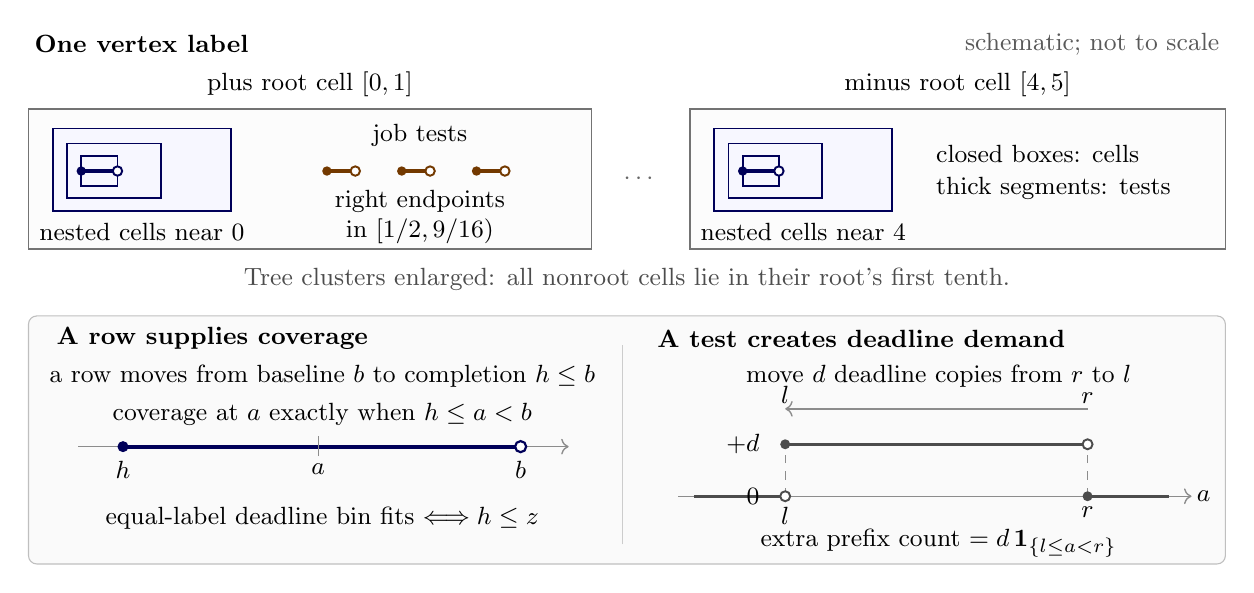
\begin{tikzpicture}[
  x=1cm,y=1cm,
  font=\fontsize{9.5}{11.5}\selectfont,
  every node/.style={inner sep=2pt},
  rootcell/.style={draw=black!55,line width=.6pt,fill=black!1},
  treecell/.style={draw=blue!35!black,line width=.65pt,fill=blue!3},
  test/.style={draw=blue!35!black,line width=1.5pt},
  jobtest/.style={draw=orange!45!black,line width=1.5pt},
  guide/.style={draw=black!45,line width=.5pt},
  heading/.style={font=\fontsize{9.5}{11.5}\selectfont\bfseries}
]
\node[heading,anchor=west] at (.15,6.65) {One vertex label};
\node[anchor=east,text=black!65] at (15.35,6.65)
  {schematic; not to scale};
\node at (3.725,6.14) {plus root cell $[0,1]$};
\node at (11.95,6.14) {minus root cell $[4,5]$};
\draw[rootcell] (.15,4.05) rectangle (7.30,5.83);
\draw[rootcell] (8.55,4.05) rectangle (15.35,5.83);
\node[text=black!60] at (7.925,4.94) {$\cdots$};

\foreach \offset in {0,8.40} {
  \begin{scope}[xshift=\offset cm]
    \draw[treecell] (.46,4.53) rectangle (2.72,5.58);
    \draw[treecell] (.64,4.70) rectangle (1.83,5.39);
    \draw[treecell] (.82,4.85) rectangle (1.28,5.23);
    \draw[test] (.82,5.04) -- (1.28,5.04);
    \fill[blue!35!black] (.82,5.04) circle (1.7pt);
    \draw[draw=blue!35!black,fill=white,line width=.7pt]
      (1.28,5.04) circle (1.7pt);
  \end{scope}
}
\node at (1.59,4.27) {nested cells near $0$};
\node at (9.99,4.27) {nested cells near $4$};
\node[align=left,anchor=west] at (11.60,5.02)
  {closed boxes: cells\\thick segments: tests};

\node at (5.12,5.50) {job tests};
\foreach \left/\right in {3.94/4.30,4.89/5.25,5.84/6.20} {
  \draw[jobtest] (\left,5.04) -- (\right,5.04);
  \fill[orange!45!black] (\left,5.04) circle (1.7pt);
  \draw[draw=orange!45!black,fill=white,line width=.7pt]
    (\right,5.04) circle (1.7pt);
}
\node at (5.12,4.66) {right endpoints};
\node at (5.12,4.27) {in $[1/2,9/16)$};
\node[text=black!70] at (7.75,3.67)
  {Tree clusters enlarged: all nonroot cells lie in their root's first tenth.};

\draw[draw=black!25,fill=black!2,rounded corners=3pt]
  (.15,.05) rectangle (15.35,3.20);
\node[heading,anchor=west] at (.43,2.91) {A row supplies coverage};
\node[heading,anchor=west] at (8.06,2.91) {A test creates deadline demand};
\draw[draw=black!20] (7.69,.30) -- (7.69,2.83);

\node at (3.88,2.43)
  {a row moves from baseline $b$ to completion $h\le b$};
\draw[guide,->] (.78,1.54) -- (7.01,1.54);
\draw[test] (1.35,1.54) -- (6.40,1.54);
\fill[blue!35!black] (1.35,1.54) circle (2pt);
\draw[draw=blue!35!black,fill=white,line width=.8pt]
  (6.40,1.54) circle (2pt);
\draw[guide] (3.83,1.42) -- (3.83,1.67);
\node[anchor=north] at (1.35,1.43) {$h$};
\node[anchor=north] at (3.83,1.40) {$a$};
\node[anchor=north] at (6.40,1.43) {$b$};
\node at (3.88,1.95) {coverage at $a$ exactly when $h\le a<b$};
\node at (3.88,.63) {equal-label deadline bin fits $\Longleftrightarrow h\le z$};

\node at (11.71,2.43) {move $d$ deadline copies from $r$ to $l$};
\draw[guide,->] (13.60,2.02) -- (9.76,2.02);
\node[anchor=south] at (9.76,2.01) {$l$};
\node[anchor=south] at (13.60,2.01) {$r$};
\draw[guide,->] (8.40,.91) -- (14.92,.91);
\draw[black!70,line width=1pt] (8.60,.91) -- (9.76,.91);
\draw[black!70,line width=1pt] (9.76,1.57) -- (13.60,1.57);
\draw[black!70,line width=1pt] (13.60,.91) -- (14.64,.91);
\draw[guide,dashed] (9.76,.91) -- (9.76,1.57);
\draw[guide,dashed] (13.60,.91) -- (13.60,1.57);
\fill[black!70] (9.76,1.57) circle (1.8pt);
\draw[black!70,fill=white,line width=.7pt]
  (13.60,1.57) circle (1.8pt);
\draw[black!70,fill=white,line width=.7pt]
  (9.76,.91) circle (1.8pt);
\fill[black!70] (13.60,.91) circle (1.8pt);
\node[anchor=east] at (9.51,1.57) {$+d$};
\node[anchor=east] at (9.51,.91) {$0$};
\node[anchor=north] at (9.76,.85) {$l$};
\node[anchor=north] at (13.60,.85) {$r$};
\node[anchor=west] at (14.91,.91) {$a$};
\node at (11.71,.31) {extra prefix count $=d\,\mathbf{1}_{\{l\le a<r\}}$};
\end{tikzpicture}
\caption{Interval coverage and deadline demand at one vertex label.
Only representative nested tree cells are shown; vertical extent
depicts containment. Leaf and job tests are left-closed and right-open.
A row with completion $h$ covers
$[h,b)$, while moving $d$ deadlines from a test's right endpoint to
its left endpoint adds exactly $d$ to the deadline prefix count on
that test. When row and unshifted-deadline baseline multisets agree,
covering every test at least $d$ times supplies the prefix inequalities
needed to match completions to deadlines.}
\label{fig:interval-mechanism}
\end{figure}


The other kind of bin pairs a job row with an anchor called a key.
Each graph edge has many repeated job positions at both endpoints.
A job row is either short or long. A long row matched to a key at
the same position must use either a limited resource called a permit
belonging to the key's edge or a resource belonging to an earlier edge.
The numerical coordinates prevent keys from using later rows or
later-edge resources. A key using an earlier row reduces the earlier
rows available for deadline bins; the resulting prefix deficit forces
additional coverage at the current job. When the plus allocation is
small, this compensation forces many exact-position long matches.
Conservation of earlier-edge resources bounds how many of those
matches can avoid the current edge's permits. If both endpoint plus
allocations were small, too many long matches would need that edge's
permits. Thus every edge has a sufficiently funded endpoint.

\paragraph{Arbitrary packings and the two consequences.}
All coordinates and subclass constraints are encoded in ordinary scalar
sizes near $1/5$. An arbitrary feasible packing need not consist of the
intended bins. Integer scores and conservation of their total leave only
a bounded number of items outside four five-item patterns. A second score
orders the vertex labels; conservation over label prefixes bounds the
number of unequal-label matches at each vertex. Crucially, the error at a
vertex is independent of the number of positions in its construction.
These bounds allow the interval and edge arguments to apply to every
packing into at most $B+c$ bins.

For completeness, a vertex cover chooses one of two local states at each
vertex, funding the plus side on the cover and the minus side elsewhere.
The cover condition ensures that all edge resources can be assigned.
For the fractional witness, instead take the four-vertex clique and give
weight one half to each local state at every vertex. Each state uses
every labeled item at its vertex exactly once, and the average demands equal
the global inventories. An explicit distribution over physical item
copies gives feasible configurations of total weight $B$. The cardinality
bound of five supplies the matching dual lower bound. This fractional
mixture does not require the states to coexist as an integral packing;
cover extraction rules out such a packing within the prescribed allowance.

Section~\ref{sec:competing-trees} proves the competing-tree lemma.
Section~\ref{sec:instance} constructs the rational item sizes and proves
their pattern, label, and order properties.
Section~\ref{sec:completeness} packs the items from a vertex cover, and
Section~\ref{sec:fractional} builds the exact fractional mixture.
Section~\ref{sec:soundness} extracts a small cover from an arbitrary packing
with extra bins. Finally, Section~\ref{sec:consequences} applies this common
reduction first to the unconditional gap and then, using H\aa stad's
satisfiability gap~\cite{Hastad2001}, to ordinary NP-hardness.

\section{Two competing trees}
\label{sec:competing-trees}

In a rooted tree $T$, the depth of a vertex is its distance from the root;
write $V_\ell(T)$ for the set of vertices at depth $\ell$.  A
\emph{marking} is a set of vertices at positive depths.  It \emph{hits} a
path if the path contains a marked vertex.  The following construction
provides two trees that each admit many hits along every path, but cannot
both be hit when their depth quotas are shared.

Depth-constrained path hitting appears in the tree formulation of resource
minimization for fire containment studied by Chalermsook and
Chuzhoy~\cite[Section~2]{ChalermsookChuzhoy2010}.
The obstruction below uses the same disjoint-branch counting principle as
their construction in Section~6: more disjoint branches than marks
available in their depth range leave one branch unhit.
Here the quotas vary with depth, and retaining paths according to their
red or blue vertex counts produces separate multiple-hit markings but
excludes a shared one-hit marking.
We prove this two-tree property in full.

\begin{lemma}[Competing trees]\label{lem:competing-trees}
For every integer $d\ge1$, there are two finite rooted trees $T^+,T^-$,
an integer $L\ge1$, and positive integer quotas $p_1,\ldots,p_L$ with the
following properties.
\begin{enumerate}[beginpenalty=10000]
\item All leaves of both trees have depth $L$.  Each tree $T^\sigma$,
$\sigma\in\{+,-\}$, has a marking $\mathcal M^\sigma$ such that
\begin{equation}\label{eq:tree-separate-marking}
 \begin{aligned}
 |\mathcal M^\sigma\cap V_\ell(T^\sigma)|&\le p_\ell
 &&(1\le\ell\le L),\\
 |\mathcal M^\sigma\cap\pi|&\ge d
 &&\text{for every root-to-leaf path $\pi$ in $T^\sigma$}.
 \end{aligned}
\end{equation}
\item For any markings $\mathcal A^+$ and $\mathcal A^-$ satisfying the
combined bounds
\begin{equation}\label{eq:tree-combined-quota}
 |\mathcal A^+\cap V_\ell(T^+)|+
 |\mathcal A^-\cap V_\ell(T^-)|\le p_\ell
 \qquad(1\le\ell\le L),
\end{equation}
at least one of the two trees has a root-to-leaf path that is not hit by
its marking.
\end{enumerate}
The trees, quotas, and separate markings are constructible by a finite
deterministic procedure depending only on $d$.
\end{lemma}

\begin{proof}
We first build one auxiliary tree $\mathcal T$, with some vertices colored
red or blue.  We then obtain $T^+$ and $T^-$ by retaining suitable complete
paths in two copies of $\mathcal T$.

\paragraph{Phases and global depths.}
Begin with a single root at depth $h_0=0$, and perform $2d-1$ phases.
At the start of phase $a$, let the current leaves be
$u_1,\ldots,u_N$, all at depth $h_{a-1}$.  The phase will add $N$ levels,
so set $h_a=h_{a-1}+N$.  Give the new global depths the quotas
\begin{equation}\label{eq:tree-phase-quotas}
 p_{h_{a-1}+i}=2^{i-1}=\frac{M_i}{2},
 \qquad M_i=2^i,\qquad 1\le i\le N.
\end{equation}
The indices $1,\ldots,N$ are local to this phase.  The successive depth
blocks $(h_{a-1},h_a]$ are disjoint, so each positive depth receives its
quota exactly once.

For each $i$, attach to $u_i$ exactly $M_i$ paths of $i$ edges, called
\emph{spines}.  They share their starting vertex $u_i$ and are otherwise
vertex-disjoint.  Color half of their endpoints red and half blue.  Each
such endpoint has depth $h_{a-1}+i$.  If $i<N$, attach to each endpoint
exactly
\begin{equation}\label{eq:tree-continuations}
 1+\sum_{j=i+1}^{N}2^{j-1}
\end{equation}
paths of $N-i$ edges, sharing only that endpoint.  Call these paths the
\emph{continuation chains}.  All vertices introduced in distinct spines
or continuation chains are new, except for the explicitly shared starting
vertices.  In particular, constructions below different $u_i$ are
disjoint.  No newly introduced vertex on a continuation chain is colored.
For $i=N$, the spine endpoint already has depth $h_a$ and no continuation
is added.

Every new leaf has depth $h_a$, and every vertex at a smaller depth has
a descendant at depth $h_a$.  This proves the equal-depth invariant for
the next phase.  After the last phase put $L=h_{2d-1}$ and let
$\mathcal T$ be the resulting tree.  All its leaves have depth $L$, and
$L\ge1$.

\paragraph{An obstruction to arbitrary markings.}
Fix any marking $\mathcal A$ of $\mathcal T$ with at most $p_\ell$ marks
at each depth $\ell$.  The marks may be anywhere at positive depths;
there is no restriction to colored vertices.  We construct a path from
the root to depth $L$ that avoids $\mathcal A$.

Suppose that a path avoiding $\mathcal A$ has reached a phase-start leaf
$u_i$.  The total number of marks anywhere in the first $i$ new levels
of this phase is at most
\begin{equation}\label{eq:tree-spine-budget}
 \sum_{j=1}^{i}p_{h_{a-1}+j}
 =\sum_{j=1}^{i}2^{j-1}
 =2^i-1=M_i-1.
\end{equation}
There are $M_i$ spines below $u_i$, disjoint after their unmarked starting
vertex.  Hitting each spine would require at least $M_i$ different marks
in these levels.  Equation~\eqref{eq:tree-spine-budget} therefore leaves
one spine entirely unmarked, including its endpoint.

If $i=N$, this spine already reaches the phase boundary.  If $i<N$, the
number of marks in all the remaining new levels is at most
$\sum_{j=i+1}^{N}2^{j-1}$.  By
Equation~\eqref{eq:tree-continuations}, the unmarked endpoint has one more
continuation chain than this bound.  The chains are disjoint after that
endpoint, so one of them is entirely unmarked.  Following it extends the
unhit path to depth $h_a$.

The root cannot be marked.  Starting there and applying this argument
through all phases gives an unhit root-to-leaf path in $\mathcal T$.
Thus no quota-respecting marking of $\mathcal T$ hits every complete path.
The argument applies to a marking fixed on the entire final tree: each
phase uses only the marks in its own block of global depths.

\paragraph{Color counts and pruning.}
At depth $h_{a-1}+i$, the only colored vertices introduced in phase $a$
are the endpoints of the $M_i$ spines below $u_i$.  Spines below the other
phase-start leaves have their endpoints at different depths, and their
descendants are disjoint from those below $u_i$.  Since the depth blocks
of different phases are disjoint, there are exactly $p_{h_{a-1}+i}$ red
vertices and the same number of blue vertices at this global depth.

Every root-to-leaf path in $\mathcal T$ encounters exactly one colored
endpoint in each phase.  It therefore contains exactly $2d-1$ colored
vertices, at least $d$ of which have the same color.  Let
$\mathcal P^+$ be the family of complete paths containing at least $d$
red vertices, and let $\mathcal P^-$ be the analogous family for blue.
These families cover all complete paths.  They are both nonempty:
at every phase-start leaf, one can choose a spine of either color and
continue to the next phase boundary, so in particular there are paths
choosing red in every phase and paths choosing blue in every phase.

In separate copies of $\mathcal T$, retain the union of the paths in
$\mathcal P^+$ and in $\mathcal P^-$, respectively; these are $T^+$ and
$T^-$.  Retain every vertex and edge on each chosen path, including
vertices with only one retained child.  No edge is contracted.  Hence
all original depths are preserved.  Every retained vertex lies on a
chosen complete path, so no vertex of depth less than $L$ becomes a leaf.
Conversely, every retained root-to-leaf path is the unique path to one
of the chosen original leaves, and thus belongs to its specified family.

Mark all retained red vertices in $T^+$ and all retained blue vertices
in $T^-$.  Pruning can only decrease their numbers at each depth.
The preceding color counts give the quotas in
Equation~\eqref{eq:tree-separate-marking}, and the definition of each
retained path family gives at least $d$ marks along every path.  All these
marks have positive depth.

\paragraph{Projection of a combined marking.}
Suppose, for a contradiction, that markings $\mathcal A^+,\mathcal A^-$
satisfy Equation~\eqref{eq:tree-combined-quota} and hit every complete path
in both trees.  Let $\varphi^\sigma:V(T^\sigma)\to V(\mathcal T)$ be the
map identifying each retained copy vertex with its original vertex, and
set
\begin{equation}\label{eq:tree-projected-marking}
 \mathcal A=
 \varphi^+(\mathcal A^+)\cup\varphi^-(\mathcal A^-).
\end{equation}
These maps preserve depths.  Taking a union merges any marks projected
onto the same original vertex, so for every $1\le\ell\le L$,
\[
 |\mathcal A\cap V_\ell(\mathcal T)|
 \le |\mathcal A^+\cap V_\ell(T^+)|
     +|\mathcal A^-\cap V_\ell(T^-)|
 \le p_\ell.
\]
The roots are unmarked, and thus $\mathcal A$ is a valid marking of
$\mathcal T$.  Every complete path in $\mathcal T$ belongs to at least
one of $\mathcal P^+,\mathcal P^-$.  Its retained copy is hit, so its
original path contains a vertex of $\mathcal A$.  This contradicts the
obstruction proved above, and establishes the combined-quota assertion.

Every phase adds finitely many explicitly specified vertices and edges.
There are finitely many phases, and the final pruning is determined by
counting colors along the finitely many complete paths.  This is a finite
deterministic construction from $d$, as claimed.
\end{proof}

\section{The reduction instance}\label{sec:instance}

\begin{theorem}[Graph-to-packing reduction]\label{thm:reduction}
Fix an integer $c\ge0$ and a real constant $\rho>0$. There is a
deterministic polynomial-time construction with the following property.
Its input is an explicitly listed simple graph $G=(V,E)$, with
$V=\{1,\ldots,n\}$ and $m=|E|\ge1$, and an integer $0\le k\le n$.
Its output is an integer $B$ and an explicit list of $5B$ rational item
sizes in $(1/6,1)$ such that:
\begin{enumerate}
 \item if $G$ has a vertex cover of size at most $k$, the items pack into
       $B$ unit-capacity bins;
 \item any packing into at most $B+c$ bins yields a vertex cover of size
       at most $k+\rho n$.
\end{enumerate}
The running-time and output-length bounds are in ordinary binary
encoding; their constants may depend on $c$ and $\rho$.
\end{theorem}

We give the construction and its elementary properties in this section.
Propositions~\ref{prop:completeness} and~\ref{prop:soundness} prove the
two implications of Theorem~\ref{thm:reduction}, respectively. Vertex
listing is part of the input representation, so the input length is at
least $n$.

\subsection{Parameters and interval geometry}

The integer $P_0$ below bounds a fixed score used to enforce the bin
patterns. The allowance $K$ will bound items lost from those patterns
when $c$ extra bins are available. Choose, once for the fixed pair
$(c,\rho)$,
\begin{equation}\label{eq:parameters}
 \begin{gathered}
  P_0=100^{11},\qquad K=25(c+1)(1+5P_0),\\
  d\in\N,\qquad d\ge\max\{72K,120K/\rho\}.
 \end{gathered}
\end{equation}
Apply Lemma~\ref{lem:competing-trees} to this $d$, obtaining
$T^+,T^-$, common leaf depth $L\ge1$, and combined depth quotas
$p_1,\ldots,p_L$. Put $P=\sum_{\ell=1}^L p_\ell$ and choose an integer
$D_*\ge1$ bounding the number of children of any node in either tree.
These quantities depend only on $c,\rho$. Set
\[
 R=100(P+nK+1).
\]
The $R$ repetitions of each incidence will make the later edge demand
larger than both the local losses $P$ and the global losses proportional
to $nK$.

Order the graph edges as $e=1,\ldots,m$. A \emph{position} is a pair
$r=(e,j)$ with $1\le j\le R$; positions are ordered lexicographically.
Define
\begin{equation}\label{eq:position-coordinates}
 \begin{aligned}
  \theta_e&=(R+1)^{e-1}-1,
  &H_{e,j}&=j(R+1)^{e-1}-1,\\
  g&=\frac{1}{16(R+1)^m},
  &b_{(e,j)}&=\frac12+gH_{e,j},\qquad \beta_e=g\theta_e.
 \end{aligned}
\end{equation}
Write $H_r=H_{e,j}$ when $r=(e,j)$. For each vertex $v$, let
\[
 \mathcal R_v=\{(e,j):v\text{ is an endpoint of }e,\ 1\le j\le R\}.
\]

Each vertex label $v$ uses its own copy of the following geometry.
The roots of $T^+$ and $T^-$ are represented by the closed side cells
$[0,1]$ and $[4,5]$. A node at depth $\ell\ge1$ has a closed cell of
width
\[
 \lambda_\ell=g[100(D_*+1)]^{-\ell}.
\]
Within a parent with left endpoint $a$, the cell of its $j$th child at
depth $\ell$ is
$[a+4j\lambda_\ell,a+(4j+1)\lambda_\ell]$.
Finally put $\Delta=\lambda_L/10$. For each $r\in\mathcal R_v$, add the
closed \emph{job cell} $[b_r-\Delta,b_r]$ on the plus side.
The \emph{test intervals} are the leaf cells of both trees and all the
job cells, each taken left-closed and right-open. Denote their union by
$\mathcal I_v$. Embedding cells remain closed whenever their geometric
intersection or containment is discussed.

\begin{lemma}[Geometry and coordinate order]\label{lem:geometry}
The embedding has the following properties.
\begin{enumerate}
 \item Every child cell lies inside its parent. Every nonroot cell lies
       in the first tenth of its root cell. Distinct depth-$\ell$ cells
       across the two trees have gaps at least $3\lambda_\ell$.
 \item The numbers $b_r$ belong to $[1/2,9/16)$, and distinct job cells
       have gaps at least $g-\Delta$. All the test intervals of one
       label are pairwise disjoint.
 \item For $1\le\ell\le L$,
       $\Delta\le\lambda_\ell/10$ and
       $\lambda_1+2\Delta<g$. An interval of length at most
       $\lambda_\ell+\Delta$ meets at most one depth-$\ell$ cell. If it
       contains a point of a leaf cell, that depth-$\ell$ cell is the
       leaf's ancestor. An interval of length at most
       $\lambda_1+\Delta$ meets at most one job cell.
 \item For $r=(e,j)$, the two independent order bounds are
       \begin{equation}\label{eq:coordinate-order}
        H_{r'}-H_r\ge\theta_e+1\quad(r'>r),\qquad
        \theta_f-\theta_e\ge H_{e,R}+1\quad(f>e).
       \end{equation}
\end{enumerate}
\end{lemma}

\begin{proof}
The right endpoint of the last child is at most
$(4D_*+1)\lambda_\ell$ beyond its parent's left endpoint. For
$\ell>1$ this is less than $\lambda_{\ell-1}$, since
$4D_*+1<100(D_*+1)$. For $\ell=1$ it is less than $g/25<1/10$.
Sibling gaps are $3\lambda_\ell$. Cells with different parents retain
at least the gap between those parents, which is at least
$3\lambda_{\ell-1}>3\lambda_\ell$; the two root cells are separated
by $3$. Induction proves the first assertion, including all cousin
cells, and descendants remain in their depth-one cells.

Successive $H$ values within edge $e$ differ by $(R+1)^{e-1}$. The
difference from $(e,R)$ to $(e+1,1)$ is the same number. Thus the first
step after a position of edge $e$ is $\theta_e+1$, proving the first
bound in Equation~\eqref{eq:coordinate-order}. Similarly,
\[
 \theta_{e+1}-\theta_e=R(R+1)^{e-1}=H_{e,R}+1,
\]
and later edges only increase this difference. Also
$0\le H_r\le R(R+1)^{m-1}-1<(R+1)^m$, proving the range of $b_r$.
Consecutive baselines differ by at least $g$, so job-cell gaps are at
least $g-\Delta$.

The widths decrease with depth, giving
$\Delta\le\lambda_\ell/10$. Since $100(D_*+1)\ge200$,
\[
 \lambda_1+2\Delta\le\frac65\lambda_1
 \le\frac{3g}{500}<g.
\]
In particular $\Delta<g\le1/16$. Job cells therefore lie strictly to
the right of $1/10$ and strictly to the left of $1$; they meet neither
tree's nonroot cells. Leaf cells have common depth $L$ and positive
gaps, proving disjointness of all tests. Finally,
$\lambda_\ell+\Delta\le(11/10)\lambda_\ell<3\lambda_\ell$, and
$\lambda_1+\Delta<g-\Delta$. These strict inequalities and the stated
gaps prove the intersection bounds. A point of a leaf belongs to its
ancestor cell at every depth, so the uniquely intersected cell at depth
$\ell$ must be that ancestor.
\end{proof}

The geometric separation has two uses. A local interval of length
$\lambda_\ell$, even with the additional shortening $\Delta$, can
intersect only one tree cell at depth $\ell$. The two coordinate-order
bounds will separately control which row positions and which edge
resources can be matched. We next realize these constraints through
five-item bins.

\subsection{Patterns and the complete item inventory}

Items have five roles: rows $X$, anchors $A$, global auxiliaries $U$,
local auxiliaries $D$, and flags $F$. Their subclasses are listed in
Table~\ref{tab:patterns}. A \emph{tuple} consists of five distinct
physical item copies. A \emph{table tuple} has one of the displayed
subclass patterns. Its kind is $\mathrm M$ for the first three rows of
Table~\ref{tab:patterns} and $\mathrm G$ for the last row. Only the roles $X,A,D$
carry vertex labels. A table tuple is \emph{good} when these three
labels are equal.

\begin{table}[htbp]
 \centering
 \begin{tabular}{c c c c c c}
  \toprule
  Kind & $X$ & $A$ & $U$ & $D$ & $F$\\
  \midrule
  $\mathrm M$ & $\Tp$ & $\Zanc$ & $\Up$ & $\DM$ & $\FT$\\
  $\mathrm M$ & $\Tm$ & $\Zanc$ & $\Um$ & $\DM$ & $\FT$\\
  $\mathrm M$ & $\Srow$ & $\Zanc$ & $\Up$ & $\DM$ & $\FM$\\
  $\mathrm G$ & $\Srow$ & $\Yanc$ & $\Waux$ & $\DG$ & $\FG$\\
  \bottomrule
 \end{tabular}
 \caption{The four table patterns, with one subclass in each role.
 Equal vertex labels on $X,A,D$ are a separate requirement for a good tuple.}
 \label{tab:patterns}
\end{table}

The $\mathrm M$ patterns will compare a row's completion with an
anchor deadline; the $\mathrm G$ pattern will match a job row to an
anchor key. The inventory below gives every role the same total count
and gives the three labeled roles the same count at each vertex.
We specify every item copy and a rational coordinate $w(i)$; the actual
size will be defined afterwards. The symbols $b,z$ and the auxiliary
lengths below are attributes of individual items.

\paragraph{Rows.}
For each label $v$ and each node of either tree, \emph{including its
root}, create $d$ rows with baseline $b$ equal to the cell's right
endpoint and coordinate $w=b$. Their subclass is $\Tp$ on the plus
side and $\Tm$ on the minus side. Add $P$ further $\Tp$ rows with
baseline $1$. Thus the tree-row counts are
\begin{equation}\label{eq:tree-row-counts}
 t_{v,+}=d|V(T^+)|+P,\qquad
 t_{v,-}=d|V(T^-)|,\qquad
 t_v=t_{v,+}+t_{v,-}\ge P+2d.
\end{equation}
For each $r\in\mathcal R_v$, create $2d$ rows of subclass $\Srow$,
all with baseline $b_r$. Of these, $d$ are \emph{short}, with
$w=b_r-\Delta$, and $d$ are \emph{long}, with $w=b_r$.
All these rows have label $v$. An intended packing sends $d$ rows at
each position to kind $\mathrm M$ and the other $d$ to kind $\mathrm G$.
Put
\[
 J_v=d|\mathcal R_v|=dR\deg(v),
\]
the number of job rows assigned to each kind in such a packing.

\paragraph{Anchors.}
For label $v$, form a baseline multiset $\mathcal B_v$ consisting of
every tree-row baseline, including padding, and $d$ copies of $b_r$
for each $r\in\mathcal R_v$. The latter are hypothetical baselines,
so $|\mathcal B_v|=t_v+J_v$, rather than the total row count.
For each test interval, replace $d$ copies of its right endpoint by
its left endpoint. Leaf-row copies and the hypothetical job copies
provide these replacements; the different tests use distinct designated
copies. For each resulting deadline $z$, create a $\Zanc$ anchor of
label $v$ with $w=-z$.

Set $\ind\{E\}=1$ when condition $E$ holds, and $0$ otherwise.
For $a\in\R$, let $B_v(a)$ be the number of members of $\mathcal B_v$
at most $a$. Moving an endpoint from $r$ to $l<r$ changes its prefix
indicator by
$\ind\{l\le a\}-\ind\{r\le a\}=\ind\{l\le a<r\}$.
Since the tests are disjoint, their deadline count satisfies exactly
\begin{equation}\label{eq:deadline-prefix}
 \#\{\Zanc\text{ anchors of label }v\text{ with }z\le a\}
 =B_v(a)+d\,\ind\{a\in\mathcal I_v\}.
\end{equation}
There are also $d$ \emph{keys} of subclass $\Yanc$ for every position
$r=(e,j)\in\mathcal R_v$, with label $v$ and coordinate
$w=-b_r-\beta_e$. Their total number is $J_v$.

\paragraph{Global auxiliaries.}
These have no vertex label. Create
$\sum_v(t_{v,+}+J_v)$ items of subclass $\Up$, exactly $dk$ of length
$1$ and the rest of length $0$. Create $\sum_v t_{v,-}$ items of
subclass $\Um$, exactly $d(n-k)$ of length $1$ and the rest of length
$0$. An item of either subclass has coordinate $w=-\len(i)$.
For each edge $e$, create $dR$ \emph{permits} of subclass $\Waux$ with
$w=\beta_e$, and $dR$ \emph{nonpermits} of that same subclass with
$w=\beta_e+\Delta$.

\paragraph{Local auxiliaries.}
For each label $v$, create $t_v+J_v$ items of subclass $\DM$.
For each $\ell=1,\ldots,L$, exactly $p_\ell$ of them have length
$\lambda_\ell$; the remaining $t_v+J_v-P$ have length $0$.
Their coordinate is $w=-\len(i)$. Also create $J_v$ items of subclass
$\DG$, with label $v$ and coordinate $0$.

\paragraph{Flags.}
Create $\sum_vt_v$ items of subclass $\FT$ and $\sum_vJ_v$ each of
subclasses $\FM$ and $\FG$. They have no vertex label and coordinate
$0$.

All multiplicities are nonnegative. In particular,
Equation~\eqref{eq:tree-row-counts} gives
$t_v+J_v-P\ge2d+J_v$ zero-length local items, while the $d$ root rows
on each side guarantee enough global items for the specified length-one
stocks, including when $k=0$ or $k=n$. Define
\begin{equation}\label{eq:inventory-total}
 B=\sum_{v=1}^n(t_v+2J_v).
\end{equation}
Each role has exactly $B$ items. This is immediate for $X,A,D$ from
their labelwise counts. For the other roles, use
$\sum_vJ_v=2dmR$: the $\Waux$ inventory is exactly $\sum_vJ_v$, and
the stated global and flag counts each sum to $B$ as well. The three
labeled roles have equal inventories $t_v+2J_v$ at every label $v$.
All coordinates satisfy $|w(i)|\le6$: cell endpoints lie in $[0,5]$,
lengths are at most $1$, and $0\le\beta_e<1/16$.

\subsection{Encoding the patterns and labels in rational sizes}

Large-base aggregation of bounded integer equations is a classical
arithmetic device; see Anthonisse~\cite[Theorem~6 and Section~5]{Anthonisse1973}.
A recent use in bin-packing constructions appears in
Jansen, Pirotton, and Tutas~\cite[Section~3]{JansenPirottonTutas2025}.
We give the bounded five-item version explicitly and separately control
the defects allowed by extra bins.

The encoding has three tasks: keep every item above $1/6$, control
departures from Table~\ref{tab:patterns}, and turn good-tuple feasibility
into an inequality on the coordinates $w(i)$. Feasibility alone will
allow some departures from the table. Conservation of the total scores
will bound their number when at most $c$ extra bins are used.

For a collection of items, let $N_s$ denote the count of subclass $s$
and $N_r$ the count of role $r$. Consider the following ten homogeneous
count equations: the five role equations
$5N_r-\sum_sN_s=0$, in the order $r=X,A,U,D,F$, followed by
\begin{equation}\label{eq:pattern-count-equations}
 \begin{aligned}
  N_{\Tp}+N_{\Tm}-N_{\FT}&=0,\\
  N_{\Zanc}-N_{\FT}-N_{\FM}&=0,\\
  N_{\Up}+N_{\Um}-N_{\FT}-N_{\FM}&=0,\\
  N_{\DM}-N_{\FT}-N_{\FM}&=0,\\
  N_{\Tm}-N_{\Um}&=0.
 \end{aligned}
\end{equation}
Here $\sum_s$ is over all thirteen subclasses. Let $\delta_j(i)$,
$0\le j<10$, be item $i$'s coefficient in these successive left sides,
and define its integer primary score by
\[
 p(i)=\sum_{j=0}^9 100^j\delta_j(i).
\]
The coefficients depend only on the subclass. Each has absolute value
at most $4$, so
$|p(i)|\le4\sum_{j=0}^9 100^j<P_0$.

For vertex labels set $Q_v=3^v$. The secondary score is $q(i)=Q_v$ for
an $X$ or $D$ item of label $v$, $q(i)=-2Q_v$ for an $A$ item of that
label, and $q(i)=0$ on the other roles. Give item $i$ the actual size
\begin{equation}\label{eq:item-size}
 \begin{gathered}
  a_i=\frac15+\gamma p(i)+\mu q(i)+\nu w(i),\\
  \gamma=\frac1{1000P_0},\qquad
  \mu=\frac{\gamma}{1000Q_n},\qquad
  \nu=\frac{\mu}{1000}.
 \end{gathered}
\end{equation}
Roles and labels specify the construction and remain available as
metadata for its analysis. The output consists of the rational sizes of
the indexed physical copies; the argument requires no recovery of this
metadata from a size and no numerical distinctness of different kinds
of items.

\begin{lemma}[Scalar encoding]\label{lem:encoding}
Every item size belongs to $(1/6,1)$, so every feasible bin has at most
five items. For a five-item tuple, zero total primary score is equivalent
to following Table~\ref{tab:patterns}. A feasible five-item tuple has
nonpositive total primary score; if that score is zero, its total
secondary score is nonpositive. If both totals are zero, feasibility is
equivalent to $\sum_iw(i)\le0$. The complete item inventory satisfies
$\sum_i p(i)=\sum_iq(i)=0$.
\end{lemma}

\begin{proof}
On a five-item tuple, every role-equation total belongs to $[-5,20]$
and each remaining total belongs to $[-5,5]$. All ten are integers of
absolute value less than $100$. If their radix-$100$ combination is
zero, reducing modulo $100$ makes the first total zero: it is a
multiple of $100$ strictly between $-100$ and $100$. Divide by $100$
and repeat to obtain all ten equations. This argument applies to signed
totals as well. The converse is immediate.

The role equations now give exactly one item of each role. With flag
$\FT$, the first subclass equation forces a tree row, the next three
force $\Zanc$, one of $\Up,\Um$, and $\DM$, and the last equation
pairs $\Tm$ precisely with $\Um$. With flag $\FM$, the row is
$\Srow$, the anchor and local item are $\Zanc,\DM$, and the global
item must be $\Up$. With flag $\FG$, the remaining subclasses are
forced to be $\Srow,\Yanc,\Waux,\DG$. These are exactly the four
patterns, each of which satisfies every equation.

The perturbation of one item from $1/5$ is bounded by
\[
 |a_i-1/5|
 \le\frac1{1000}+\frac{2}{10^6P_0}
       +\frac{6}{10^9P_0Q_n}<\frac1{30}.
\]
Thus $a_i>1/6$ and $a_i<7/30<1$. For five items, the total absolute
contribution below the primary scale is at most
$10Q_n\mu+30\nu$, and
\[
 \frac{10Q_n\mu+30\nu}{\gamma}
 =\frac1{100}+\frac{3}{100000Q_n}<1,
 \qquad \frac{30\nu}{\mu}=\frac3{100}<1.
\]
An integer primary total at least $1$ would therefore make the bin's
size exceed $1$. If the primary total is zero, the same argument at
the secondary scale excludes a positive secondary total. When both
vanish, the five copies of $1/5$ already sum to $1$, leaving exactly
the asserted coordinate condition.

Finally, the whole inventory satisfies all ten count equations. Every
role has $B$ items; the tree-row and $\FT$ counts both equal
$\sum_vt_v$; each of the $\Zanc$, combined $\Up,\Um$, and $\DM$
counts equals $\sum_v(t_v+J_v)$; and the $\Tm$ and $\Um$ counts
agree. Thus the primary total is zero. At each label the $X,A,D$
inventories are equal, so its secondary contribution is
$(1-2+1)Q_v(t_v+2J_v)=0$.
\end{proof}

\paragraph{Polynomial construction.}
For fixed $c,\rho$, the trees and all their parameters are finite
constants. In particular $t_v=t$ is a fixed constant, while
$R=O(n+1)$ and
$B=nt+4dmR$. Hence all positions and all item copies can be enumerated
in polynomial time in the explicit graph input. The denominators
\begin{equation}\label{eq:encoding-denominators}
 \begin{aligned}
  D_{\rm geom}&=160(R+1)^m[100(D_*+1)]^L,\\
  D_{\rm size}&=10^9P_0 3^n D_{\rm geom}
 \end{aligned}
\end{equation}
are common denominators for all coordinates $w(i)$ and all sizes $a_i$,
respectively. Indeed, $D_{\rm geom}$ accommodates $g$, every
$\lambda_\ell$, $\Delta$, all nested endpoints, and every baseline and
$\beta_e$; Equation~\eqref{eq:item-size} then gives the second claim.
Their bit lengths are
$O(n+m\log(n+2))$, with constants depending on the fixed parameters.
Since $0<a_i<1$, numerators over $D_{\rm size}$ have the same bound.
Integer powering, arithmetic, item enumeration, and optional fraction
reduction therefore take polynomial bit time. The choice of $d$ and the
finite tree construction are fixed for each reduction; $\rho$ is not a
real-valued runtime input.

\begin{lemma}[Good anchors under an additive allowance]\label{lem:good-anchors}
In any packing of the constructed instance into at most $B+c$ bins,
fewer than $K$ items lie outside five-item table tuples. At each vertex
label $v$, at most $3K$ anchors lie outside good tuples. This is a joint
bound on its $\Zanc$ and $\Yanc$ anchors, and therefore applies to any
subset of that label's anchors.
\end{lemma}

\begin{proof}
If the packing has $N\le B+c$ bins, five-item capacity gives $N\ge B$.
The number of unused five-item slots is $5(N-B)\le5c$. Hence there
are at most $5c$ nonfull bins and at most $25c$ items in them. All full
bins have nonpositive integer primary totals by
Lemma~\ref{lem:encoding}. The whole primary total is zero, so the
sum of the magnitudes of the negative full-bin totals is at most
$25cP_0$, supplied by the nonfull items. There are consequently at most
$25cP_0$ negative-primary full bins. The number of items outside
primary-zero full bins is at most
\begin{equation}\label{eq:primary-loss}
 25c+5(25cP_0)=25c(1+5P_0)<K.
\end{equation}
Those primary-zero bins are precisely the table tuples.

In a table tuple write $v_X,v_D,v_A$ for its three labels. Its
secondary score is
$Q_{v_X}+Q_{v_D}-2Q_{v_A}\le0$. If $v_X>v_A$, then
$Q_{v_X}\ge3Q_{v_A}$, already exceeding the negative contribution;
the same argument applies to $v_D$. Thus
\[
 v_X\le v_A,\qquad v_D\le v_A.
\]
Equality of the secondary total occurs exactly when all three labels
are equal.

Here is the exact conservation law that controls smaller-label imports.
Fix a prefix $S=\{1,\ldots,h\}$ and a role $r\in\{X,D\}$.
Let $O_A(S)$ and $O_r(S)$ count items of the indicated role and labels
in $S$ outside table tuples. Let $E_r(S)$ count table tuples whose
role-$r$ item has label in $S$ and whose anchor has label outside $S$.
The original inventories of either role in $S$ equal
$\sum_{v\in S}(t_v+2J_v)$. Every table anchor in $S$ consumes a
role-$r$ item in $S$. Subtracting this consumption from the available
role-$r$ items gives
\begin{equation}\label{eq:label-prefix-conservation}
 E_r(S)=O_A(S)-O_r(S)\le O_A(S)\le K.
\end{equation}
This identity also holds for the empty prefix.

For anchors of label $v$, any unequal row label must be below $v$ and
is counted by $E_X(\{1,\ldots,v-1\})$. At most $K$ table anchors
of label $v$ have this defect. At most another $K$ have a smaller
local-auxiliary label. At most $K$ anchors of the label lie outside
table tuples altogether. Their union has at most $3K$ members, proving
the joint assertion. Summing this bound over labels permits a global
loss of $3nK$.
\end{proof}

\subsection{Feasibility of good tuples}

Lemma~\ref{lem:good-anchors} now lets us analyze an arbitrary packing
through its good tuples, losing at most $3K$ anchors at each vertex.
The loss is independent of the number of job positions. For good
tuples, the remaining coordinate inequality has the following concrete
meaning.

\begin{lemma}[Completion and key inequalities]\label{lem:good-feasibility}
A good tuple has zero primary and secondary totals. Its feasibility is
therefore described exactly as follows.
\begin{enumerate}
 \item For kind $\mathrm M$, with row baseline $b$, deadline $z$,
       and associated global and local items $U,D$, define
       \begin{equation}\label{eq:completion-coordinate}
        h=b-\Delta\ind\{\text{row is short}\}-\len(U)-\len(D).
       \end{equation}
       The tuple is feasible if and only if $h\le z$, and $h\le b$.
       For any collection of such row--auxiliary assignments and any
       $a\in\R$,
       \begin{equation}\label{eq:completion-prefix}
        \#\{h\le a\}=\#\{b\le a\}+\#\{h\le a<b\}.
       \end{equation}
       The last term counts coverage by the half-open intervals $[h,b)$.
 \item For kind $\mathrm G$, let its key have position $r=(e,j)$,
       its row have position $r'$, and its global item belong to edge
       $f$. Feasibility is equivalent to
       \begin{equation}\label{eq:key-feasibility}
        b_{r'}-b_r+\beta_f-\beta_e
        +\Delta\bigl(\ind\{\text{nonpermit}\}
                      -\ind\{\text{row is short}\}\bigr)\le0.
       \end{equation}
       It implies both $r'\le r$ and $f\le e$. For an exact-position
       long row, the global item must be a permit of edge $e$ or an
       item of an earlier edge. At the exact position and edge, a
       short row admits either a permit or a nonpermit, whereas a long
       row admits only a permit.
\end{enumerate}
\end{lemma}

\begin{proof}
The table pattern gives zero primary score; equal labels give
$Q_v+Q_v-2Q_v=0$. Apply Lemma~\ref{lem:encoding}. In kind
$\mathrm M$, the five coordinates sum to $h-z$, proving the first
criterion. All lengths and the shortening term are nonnegative, so
$h\le b$. The events $\{b\le a\}$ and $\{h\le a<b\}$ partition
$\{h\le a\}$, proving Equation~\eqref{eq:completion-prefix}, including
the endpoints and the empty intervals when $h=b$.

In kind $\mathrm G$, summing the row, key, global, local, and flag
coordinates gives exactly the left side of
Equation~\eqref{eq:key-feasibility}. If $r'>r$, then
Equation~\eqref{eq:coordinate-order} gives a position increase at least
$g(\theta_e+1)$. Since $\theta_f\ge0$, the $\beta$ difference is at
least $-g\theta_e$. The final perturbation is at least $-\Delta$.
The total is therefore at least $g-\Delta>0$, excluding $r'>r$
without any condition on $f$.

Independently, if $f>e$, the $\beta$ increase is at least
$g(H_{e,R}+1)$. Since $H_{r'}\ge0$ and $H_r\le H_{e,R}$, the
position difference is at least $-gH_{e,R}$. Again the total is at
least $g-\Delta>0$, excluding $f>e$ without any condition on $r'$.
For an exact-position long row, a same-edge nonpermit would leave
the strictly positive sum $\Delta$, proving the resource restriction.
For an exact-position, same-edge tuple, the sum is simply
$\Delta(\ind\{\text{nonpermit}\}-
\ind\{\text{row is short}\})$, which gives the remaining assertions.
\end{proof}

For later geometric use, an $\mathrm M$ interval with global length
zero and local length $\lambda_\ell$ has length at most
$\lambda_\ell+\Delta$. With both lengths zero it is empty, except
for a short $\Srow$ row, whose interval is its job test interval.
Thus the intersection bounds of Lemma~\ref{lem:geometry} apply even
when the row's baseline is unrelated to the depth of its local item.
Finally, a plus row has $b\le1$, while a minus row has $b\ge4$ and
is never short. Subtracting a global length at most $1$ and a local
length at most $\lambda_1<1/10$ leaves its completion greater than
$1$. Consequently intervals on either side can cover test points
only on that side.

\section{Packing from a vertex cover}\label{sec:completeness}

\begin{proposition}\label{prop:completeness}
If the input graph has a vertex cover of size at most $k$, the constructed
items can be packed into $B$ bins.
\end{proposition}

\begin{proof}
Enlarge the cover to a set $C\subseteq V$ of exactly $k$ vertices.
Call vertices of $C$ \emph{selected} and the others \emph{unselected}.
We first construct the $\mathrm M$ bins separately at each vertex.
The local construction will also be useful when no common cover is
specified.

\paragraph{Rows and auxiliary slots.}
At label $v$, put every $\Tp$ and $\Tm$ row into $\mathrm M$.
At each position in $\mathcal R_v$, put the $d$ long $\Srow$ rows
into $\mathrm M$ if $v$ is selected, and the $d$ short rows otherwise.
There are $t_v+J_v$ such rows, hence this many slots for each of
$\Zanc$ and $\DM$.
The roots and padding give the useful bound
\begin{equation}\label{eq:local-slot-bound}
 t_v=P+d\bigl(|V(T^+)|+|V(T^-)|\bigr)\ge P+2d.
\end{equation}
In particular the number of zero-length $\DM$ copies is
$t_v+J_v-P\ge2d+J_v$.

At a selected vertex, choose $d$ distinct plus-root rows and give
them length-one $\Up$ items; at an unselected vertex do the same
with minus-root rows and length-one $\Um$ items.  Reserve $d$
zero-length $\DM$ copies for these funded rows.
Every other $\mathrm M$ row receives a length-zero global auxiliary:
$\Tp$ and $\Srow$ require $\Up$, and $\Tm$ requires $\Um$.
Thus label $v$ has $t_{v,+}+J_v$ plus slots and $t_{v,-}$ minus
slots.  Globally the requested length-one counts are exactly $dk$
and $d(n-k)$; the total slots are precisely the respective global
inventories.  Consequently all global auxiliaries of these two
subclasses can be assigned as distinct physical copies, exhausting
their length-one and length-zero stocks.

In the tree on the unfunded side, choose the separate $d$-fold
marking from Lemma~\ref{lem:competing-trees}.  For every marked
depth-$\ell$ vertex, choose one of its $d$ endpoint rows and attach
a $\DM$ item of length $\lambda_\ell$.  The depth quota supplies
enough such items.  These marked rows are distinct and have positive
depth, so none is a funded-root row.  If $s_v$ nodes are marked, then
$s_v\le P$.  After these assignments and the reserved root zeros,
there are $t_v+J_v-s_v-d$ unassigned local slots.  By
Equation~\eqref{eq:local-slot-bound}, this is at least $P-s_v$, the
number of unused positive local items.  Put those items in distinct
remaining slots, then fill all other slots with the remaining zeros.
This uses every $\DM$ copy.  All additional positive lengths move
their rows earlier and cannot remove any coverage already obtained.
The same argument applies when $v$ is isolated and $J_v=0$.

Attach a $\FT$ flag to every tree row and a $\FM$ flag to every
$\Srow$ row used here.  These requests exhaust the $\FT$ and $\FM$ inventories
after summing over labels.  From now on keep each row, its two
auxiliaries, and its flag together.

\paragraph{Coverage and deadlines.}
For each such group, let $b$ be its row baseline and let
\[
 h=b-\Delta\ind\{\text{row is short}\}
      -\len(U)-\len(D)
\]
be its completion coordinate, as in
Lemma~\ref{lem:good-feasibility}.  Always $h\le b$.
Each funded-root row covers $[0,1)$ or $[4,5)$ through its interval
$[h,b)$.  Hence the $d$ funded roots cover every test interval on
that side $d$ times, including all job intervals when plus is funded.
At a marked depth-$\ell$ node on the other side, the assigned local
length gives precisely its cell with the right endpoint removed.
By nesting in Lemma~\ref{lem:geometry}, this interval contains the
test interval of every descendant leaf.  The $d$-fold marking covers every leaf test on that
side at least $d$ times.  Finally, at an unselected vertex each job
has $d$ short rows in $\mathrm M$; even before any auxiliary
shortening they cover its interval $[b_r-\Delta,b_r)$.
Thus every test interval receives at least $d$ covering intervals
in either state.

The baseline multiset of these $\mathrm M$ rows is exactly the one
defining $B_v(a)$: all tree baselines and $d$ copies of $b_r$ at
each job, irrespective of the choice of short or long rows.
Recall that $\mathcal I_v$ is the union of the test intervals at $v$.
For every real $a$,
\begin{equation}\label{eq:complete-prefix}
 \#\{h\le a\}
 =B_v(a)+\#\{h\le a<b\}
 \ge B_v(a)+d\ind\{a\in\mathcal I_v\}.
\end{equation}
The last expression is the exact number of deadlines at most $a$.
Here the left-closed, right-open convention includes a shifted
deadline at the left endpoint and stops counting the extra copy
when its original baseline enters at the right endpoint.

Sort the completions as $h_1\le\cdots\le h_{t_v+J_v}$ and the
deadlines as $z_1\le\cdots\le z_{t_v+J_v}$, retaining the identity
of each copy.  Equation~\eqref{eq:complete-prefix} at $a=z_j$
shows $h_j\le z_j$.  Attach the $j$th deadline anchor to the group
with completion $h_j$.
Only the $\Zanc$ anchors are permuted; the row, global auxiliary,
local auxiliary, and flag stay together.  All the anchors have the
same subclass and label $v$, so every resulting tuple keeps its
required pattern and equal labels.  Its deadline inequality makes
it feasible by Lemma~\ref{lem:good-feasibility}.

\paragraph{The remaining rows and edge resources.}
At each incidence position, pair its remaining $d$ rows with its
$d$ keys, using the exact position and label.  Add distinct $\DG$
copies of that label and $\FG$ flags.  The remaining rows are short
at a selected vertex and long at an unselected vertex.
For a $\Waux$ item of the exact edge, the coordinate condition in
Lemma~\ref{lem:good-feasibility} reduces to
\begin{equation}\label{eq:exact-edge-completeness}
 \Delta\bigl(\ind\{\text{nonpermit}\}
                 -\ind\{\text{row is short}\}\bigr)\le0.
\end{equation}
Thus a long row requires a permit, whereas a short row accepts
either species.

Each endpoint of an edge has $dR$ such slots.  If exactly one
endpoint is unselected, assign all $dR$ permits to its long rows
and all $dR$ nonpermits to the selected endpoint's short rows.
If both endpoints are selected, all $2dR$ rows are short; assign
the $dR$ permits and the $dR$ nonpermits to these slots in any order.
Since $C$ is a cover, these are the only cases.  In both cases
every $\Waux$ copy is used, and all $\mathrm G$ tuples are feasible.

At label $v$ we have made $t_v+J_v$ bins of type $\mathrm M$ and
$J_v$ of type $\mathrm G$.  They use every labeled row, anchor,
and local auxiliary once.  Their flag counts are $t_v$ of $\FT$
and $J_v$ each of $\FM$ and $\FG$, and all global inventories have
been exhausted.  Every bin follows Table~\ref{tab:patterns} and
has equal labels, so Lemmas~\ref{lem:encoding} and
\ref{lem:good-feasibility} apply to the actual encoded sizes.
The construction is a partition of all items into
$\sum_v(t_v+2J_v)=B$ feasible bins.
\end{proof}

\section{The fractional packing}\label{sec:fractional}

We construct a fractional packing of value $B$ for the four-vertex
instance. Both configuration models are those of
Definition~\ref{def:configuration-lp}; all feasible configurations are
allowed, with no restriction to the table patterns used in our witness.
The matching lower bound will follow from the five-item capacity limit.

\begin{proposition}\label{prop:fractional}
For the instance constructed from the complete graph on four
vertices with $k=2$, using the parameters in
Equation~\eqref{eq:parameters}, both configuration relaxations have
value $B$:
\[
 \OPT_{\mathrm{LP,ind}}=\LP=B.
\]
\end{proposition}

\begin{proof}
For each label $v$, construct the local groups from the proof of
Proposition~\ref{prop:completeness} twice, once selected and once
unselected.  In the selected state, put short rows in $\mathrm G$
and require only nonpermits of the exact edge.  In the unselected
state, put long rows there and require only permits of the exact
edge.  Equation~\eqref{eq:exact-edge-completeness} holds with
equality in both states.
The local $\mathrm M$ construction and deadline matching did not
use neighboring states.  Each state therefore gives a collection
of $N_v=t_v+2J_v$ feasible bin templates, using every physical
copy in the labeled roles $X,A,D$ exactly once.
Fix these labeled assignments in both states, including the local
auxiliaries and the independently sorted anchors.  The two remaining
slots in a template specify a global-auxiliary species and a flag
species.

\paragraph{Exact resource demands.}
Table~\ref{tab:local-state-demands} lists the required counts.
The two $\Waux$ rows refer to each edge $e$ incident to $v$.
\begin{table}[htbp]
\centering
\caption{Pooled-item demands at one vertex in the two local states.}
\label{tab:local-state-demands}
\vspace{6pt}
\begin{tabular}{@{}lccc@{}}
\toprule
Species & Selected & Unselected & Half of each\\
\midrule
$\Up$, length $1$ & $d$ & $0$ & $d/2$\\
$\Up$, length $0$ & $t_{v,+}+J_v-d$ & $t_{v,+}+J_v$
 & $t_{v,+}+J_v-d/2$\\
$\Um$, length $1$ & $0$ & $d$ & $d/2$\\
$\Um$, length $0$ & $t_{v,-}$ & $t_{v,-}-d$ & $t_{v,-}-d/2$\\
$\Waux$, permit of $e$ & $0$ & $dR$ & $dR/2$\\
$\Waux$, nonpermit of $e$ & $dR$ & $0$ & $dR/2$\\
$\FT$ & $t_v$ & $t_v$ & $t_v$\\
$\FM$ & $J_v$ & $J_v$ & $J_v$\\
$\FG$ & $J_v$ & $J_v$ & $J_v$\\
\bottomrule
\end{tabular}
\end{table}

Each entire local state can in fact choose distinct pooled copies
from the actual inventories.  Both length-one pools have $2d$
copies, while a state needs at most $d$ of either.
Every other vertex contributes at least $d$ root slots on each
side, so the zero-length stocks satisfy
\begin{align*}
 \sum_w(t_{w,+}+J_w)-2d&\ge t_{v,+}+J_v+d,\\
 \sum_w t_{w,-}-2d&\ge t_{v,-}+d.
\end{align*}
These bounds exceed the respective largest local demands.
Each permit or nonpermit pool of an incident edge has exactly
$dR$ copies, enough for its local demand, and each flag pool
contains at least the number required at one vertex.  All pools
requested by any template are therefore nonempty.  Different
local states may reuse copies; we will now allocate their
fractional uses explicitly.

Taking half of both states at every vertex gives total demand equal
to every pooled stock.
Indeed, summing over the four vertices gives $2d$ length-one
items on each side and exactly the prescribed zero-length counts.
Each edge has two endpoints, which together request $dR$ permits
and $dR$ nonpermits.  Each flag has the same demand in both states,
so its weighted total is also its inventory.

\paragraph{Columns using physical copies.}
For a template $b$, let $i_b^X,i_b^A,i_b^D$ be its fixed labeled
copies.  Let $\mathcal U_b$ be the set of physical copies in its
required global species, distinguishing side and length for
$\Up,\Um$, and edge and permit status for $\Waux$.
Let $\mathcal F_b$ be the set of copies of its required flag.
For every pair $(u,f)\in\mathcal U_b\times\mathcal F_b$, assign
the individual-copy configuration
\begin{equation}\label{eq:physical-fractional-columns}
 H_{b,u,f}=\{i_b^X,i_b^A,u,i_b^D,f\}
 \quad\text{weight}\quad
 \frac{1}{2|\mathcal U_b|\,|\mathcal F_b|}.
\end{equation}
Do this for every template in both states of every vertex, adding
weights whenever the same configuration is generated more than once.
All five physical copies in a column are distinct because their
roles are disjoint.  Copies within either requested pool have
identical encoded sizes; hence every generated column is feasible.
Coincidences of numerical sizes between different declared species
do not affect their disjoint physical indices or this argument.

The columns generated by one template have total weight $1/2$.
Every labeled item occurs in one template in each of its two local
states, giving total coverage $1$.
For a global pool $\mathcal U$, each requesting template contributes
$1/(2|\mathcal U|)$ to each copy's coverage after summing over flag
choices.  Its total half-weight demand equals $|\mathcal U|$, as
just proved, so each global copy also has coverage $1$.
The same calculation, summing over global choices, gives coverage
$1$ for each flag copy.  Equation~\eqref{eq:physical-fractional-columns}
therefore defines a feasible solution of
Equation~\eqref{eq:individual-configuration-lp}, with objective
\[
 \sum_{v=1}^4\left(\frac{N_v}{2}+\frac{N_v}{2}\right)=B.
\]

Project each individual configuration to its vector of multiplicities
of equal numerical sizes, and sum the weights of configurations
with the same vector.  Capacity is unchanged, and summing the
individual coverage equalities over copies of a given size gives
its required multiplicity.  This proves $\LP\le B$ for the ordinary
type LP, including when different species have equal sizes.

Finally, Lemma~\ref{lem:encoding} gives $a_i>1/6$ for every item.
Every feasible configuration consequently has cardinality at most
five, counting multiplicity in the type formulation.  Giving dual
weight $1/5$ to every physical item, or to every numerical size
type, is therefore feasible for the respective covering LP.
Both dual objectives equal $|\mathcal I|/5=5B/5=B$.
Thus both relaxations have value exactly $B$.

This construction uses feasible local bin configurations.  It does
not require a vertex cover of size two in the four-vertex clique,
nor an integral packing obtained by making those local choices
simultaneously.  The integral lower bound will follow separately
from Proposition~\ref{prop:soundness}.
\end{proof}

\section{Extracting a small vertex cover}\label{sec:soundness}

\begin{proposition}[Soundness]\label{prop:soundness}
If the instance of Theorem~\ref{thm:reduction} packs into at most
\(B+c\) bins, then its input graph has a vertex cover of size at most
\(k+\rho n\).
\end{proposition}

We first use deadline prefixes to force coverage at every test point.
The competing trees then force a large global allocation on one side
of each vertex. Repeated edge jobs turn the plus allocations into a
vertex cover, whose size is bounded by the global item inventories.

Fix such a packing throughout this section.  By
Lemma~\ref{lem:good-anchors}, at most \(3K\) anchors of any fixed label
fail to belong to good tuples.  This bound applies to every subset of
that label's anchors, including any chosen collection of deadlines or
keys.  Summing over labels gives a bound of \(3nK\) when needed.

Let \(\mathcal M_v\) be the set of good \(\mathrm M\) tuples of label
\(v\).  Each has a row baseline \(b\), a completion coordinate \(h\le b\),
and the associated coverage interval \([h,b)\).
Write \(x_v^+\) and \(x_v^-\) for the numbers of these tuples using,
respectively, a length-one \(\Up\) or \(\Um\) item.  Distinct tuples
use distinct items, so the inventories give
\begin{equation}\label{eq:sound-global-budgets}
 \sum_v x_v^+\le dk,\qquad
 \sum_v x_v^-\le d(n-k),\qquad
 \sum_v(x_v^++x_v^-)\le dn.
\end{equation}
All interval counts below include multiplicities of tuples.

\subsection{Coverage and a forced side}

For a real point \(a\), define
\[
 A_v(a)=\#\{M\in\mathcal M_v:b(M)\le a\},\qquad
 C_v(a)=\#\{M\in\mathcal M_v:h(M)\le a\},
\]
and let \(I_v(a)\) count the intervals of \(\mathcal M_v\) containing
\(a\).  Because \(h\le b\), the identity
\(\ind\{h\le a\}=\ind\{b\le a\}+\ind\{h\le a<b\}\)
holds even at tied endpoints.  Consequently
\begin{equation}\label{eq:sound-prefix-decomposition}
 C_v(a)=A_v(a)+I_v(a).
\end{equation}
The function \(B_v(a)\) remains the original baseline prefix used to
define the deadlines; it need not equal \(A_v(a)\) in this packing.

\begin{lemma}[Coverage at every test point]\label{lem:coverage}
For every label \(v\) and every point \(a\) in one of its half-open
test intervals,
\begin{equation}\label{eq:sound-test-coverage}
 I_v(a)\ge d-6K.
\end{equation}
\end{lemma}

\begin{proof}
There are exactly \(B_v(a)+d\) deadlines at most \(a\).
At least \(B_v(a)+d-3K\) of their anchors are good.
Their distinct \(\mathrm M\) matches have \(h\le z\le a\) by
Lemma~\ref{lem:good-feasibility}, giving
\begin{equation}\label{eq:sound-completion-prefix}
 C_v(a)\ge B_v(a)+d-3K.
\end{equation}
The deadline formula uses the half-open test convention: moving
\(d\) copies from a right endpoint \(r_0\) to a left endpoint
\(\ell_0\) changes the prefix by
\(d(\ind\{\ell_0\le a\}-\ind\{r_0\le a\})
=d\ind\{\ell_0\le a<r_0\}\).

Let \(N'\) be the number of positions in \(\mathcal R_v\) with
\(b_r\le a\).  There are \(2dN'\) actual \(\Srow\) rows at those
positions and \(dN'\) keys there.  At least \(dN'-3K\) of these keys
have good \(\mathrm G\) matches.  The row-order conclusion of
Lemma~\ref{lem:good-feasibility} places all their rows in this same
baseline prefix.  Since these are distinct rows, at most
\[
 2dN'-(dN'-3K)=dN'+3K
\]
of the prefix's \(\Srow\) rows can occur in good \(\mathrm M\)
tuples.  This inequality is valid also when \(dN'-3K<0\).
Other uses of prefix rows only reduce the number available.
The \(\Tp,\Tm\) rows contribute at most their entire original
baseline prefix.  Since \(B_v(a)\) includes exactly \(dN'\)
hypothetical job baselines, we obtain
\begin{equation}\label{eq:sound-baseline-prefix}
 A_v(a)\le B_v(a)+3K.
\end{equation}
Subtracting Equation~\eqref{eq:sound-baseline-prefix} from
Equation~\eqref{eq:sound-completion-prefix} and using
Equation~\eqref{eq:sound-prefix-decomposition} proves the claim.
\end{proof}

\begin{lemma}[A large count on one side]\label{lem:side-choice}
Every vertex \(v\) satisfies
\begin{equation}\label{eq:sound-side-choice}
 x_v^+\ge d-6K\qquad\text{or}\qquad x_v^-\ge d-6K.
\end{equation}
\end{lemma}

\begin{proof}
A length-one global item can contribute coverage only on its own
side.  Indeed, a minus row has baseline at least \(4\), is not short,
and has completion at least \(4-1-\lambda_1>1\).
Every plus row, including each \(\Srow\) row, has baseline at most
\(1\), so its interval cannot cover a minus test point.

Choose one interior point in each tree leaf cell.  A tuple whose
global and local lengths are both zero has an empty interval unless
its row is short.  In the latter case its interval is exactly its
job test interval, which is disjoint from all leaf cells.
For a tuple with global length zero and positive local length
\(\lambda_\ell\), the interval length is at most
\[
 \lambda_\ell+\Delta\le \frac{11}{10}\lambda_\ell<3\lambda_\ell.
\]
By Lemma~\ref{lem:geometry}, it therefore meets at most one closed
depth-\(\ell\) cell across the two trees.  If there is such a cell,
mark its tree vertex.  In particular, if the interval covers a
chosen leaf point, that point belongs to its depth-\(\ell\)
ancestor cell; the marked vertex is this ancestor.
This reasoning depends on the interval's length, regardless of
the row's baseline or depth.

Make these marks for all global-zero, positive-local tuples of
label \(v\), merging repeated marks at the same tree vertex.
At depth \(\ell\), the number of marks across both trees is at most
the number of used length-\(\lambda_\ell\) local items, hence at
most \(p_\ell\).  All marks are at positive depths.  The retained
depths in Lemma~\ref{lem:competing-trees} ensure that every leaf has
the ancestor used above.

If both counts in Equation~\eqref{eq:sound-side-choice} were less
than \(d-6K\), Lemma~\ref{lem:coverage} would force every chosen
leaf point to be covered by some global-zero, positive-local tuple.
The marks would then hit every root-to-leaf path in both trees,
contrary to the combined-quota obstruction of
Lemma~\ref{lem:competing-trees}.
\end{proof}

\subsection{Job positions and displaced rows}

The forced side at each vertex does not yet ensure that every graph
edge is covered. We must connect the plus allocation to the incident
jobs. A key may use an earlier row, so this connection requires an
explicit count of displaced rows rather than an assumption of
position-by-position matching.

For each label \(v\), exclude a position \(r\in\mathcal R_v\)
if its closed job cell \([b_r-\Delta,b_r]\) meets a coverage interval
from a good \(\mathrm M\) tuple of that label with global length zero
and positive local length.  This definition uses closed cells;
the tested coverage intervals remain half-open.
Such a tuple's interval has length at most
\(\lambda_1+\Delta<g-\Delta\), by
Lemma~\ref{lem:geometry}.  Distinct job cells have gap at least
\(g-\Delta\), so the interval meets at most one of them.
There are at most \(P\) positive local items of label \(v\).
Thus at most \(P\) positions are excluded in all of
\(\mathcal R_v\), and each incident edge retains at least \(R-P\)
nonexcluded positions.

For \(r\in\mathcal R_v\), let \(L_{v,r}\) be the number of good
\(\mathrm G\) tuples whose key is at \(r\) and whose row is a long
row of that same position.

\begin{lemma}[Long matches at a nonexcluded job]\label{lem:job-matches}
Every nonexcluded position \(r\in\mathcal R_v\) satisfies
\begin{equation}\label{eq:sound-long-matches}
 L_{v,r}\ge d-x_v^+-9K.
\end{equation}
\end{lemma}

\begin{proof}
Test at the interior point \(a=b_r-\Delta/2\).
Since position gaps are at least \(g>\Delta\), the job baselines
at most \(a\) are exactly those at positions strictly earlier than
\(r\).  Let \(N'\) count those positions, and let \(\xi\) count
the good tuples whose key is at \(r\) and whose row is from a
strictly earlier position.

The good keys at earlier positions consume at least \(dN'-3K\)
distinct rows from the earlier prefix, by the same order argument
as in Lemma~\ref{lem:coverage}.  The \(\xi\) current-key matches
consume an additional \(\xi\) rows from that prefix: their keys
are distinct from the earlier keys, and a packing cannot use one
row in two tuples.  Among its \(2dN'\) rows, at most
\(dN'+3K-\xi\) can therefore appear in good \(\mathrm M\) tuples.
Including the original tree-row prefix gives the strengthened bound
\begin{equation}\label{eq:sound-displaced-prefix}
 A_v(a)\le B_v(a)+3K-\xi.
\end{equation}

Let \(u\) count the short rows of the current position \(r\) used
in good \(\mathrm M\) tuples.  Every interval covering \(a\)
is accounted for as follows:
\begin{itemize}
 \item Tuples with global length one contribute at most \(x_v^+\)
 in total, since minus tuples cannot reach this plus-side point.
 \item A global-zero tuple with positive local length contributes
 nothing, since the position was not excluded.
 \item With both lengths zero, a tree row or a long job row has
 an empty interval.  A short row covers only its own job interval,
 so it can cover \(a\) only at the current position.
\end{itemize}
It follows that
\begin{equation}\label{eq:sound-job-coverage-upper}
 I_v(a)\le x_v^++u.
\end{equation}
A current short row with global length one may be counted in
both \(x_v^+\) and \(u\); this only enlarges the upper bound.

Combine Equations~\eqref{eq:sound-prefix-decomposition},
\eqref{eq:sound-completion-prefix},
\eqref{eq:sound-displaced-prefix}, and
\eqref{eq:sound-job-coverage-upper} to obtain
\[
 B_v(a)+d-3K
 \le B_v(a)+3K-\xi+x_v^++u.
\]
Equivalently,
\begin{equation}\label{eq:sound-xi-correction}
 u-\xi\ge d-x_v^+-6K.
\end{equation}
Here the same \(3K\) loss controls the entire earlier-key prefix;
it is not incurred separately at its positions.

At least \(d-3K\) keys at \(r\) are in good tuples.
Exactly \(\xi\) of the good matches use earlier rows, and the
row-order restriction forces every other good match to use a row
at \(r\).  At most \(d-u\) of the short rows there are available
to these matches, because \(u\) have already been used in good
\(\mathrm M\) tuples.  Any other use of a short row only lowers
this availability.  Hence
\[
 L_{v,r}\ge d-3K-\xi-(d-u)
          =u-\xi-3K
          \ge d-x_v^+-9K,
\]
as required.
\end{proof}

\subsection{Edge capacity and the threshold cover}

\begin{lemma}[The threshold set covers every edge]\label{lem:edge-cover}
The set
\[
 C=\{v:x_v^+>d/8\}
\]
is a vertex cover.
\end{lemma}

\begin{proof}
Fix an edge index \(e\), with endpoints \(v_1,v_2\).
There are exactly \(2dR(e-1)\)
\(\Waux\) items belonging to earlier edges, counting both permits
and nonpermits.  This equals the total number of earlier-edge
keys over all labels, since each edge has two endpoints.
At least \(2dR(e-1)-3nK\) of those keys are in good tuples.
By the edge-order conclusion of Lemma~\ref{lem:good-feasibility},
each consumes a distinct \(\Waux\) item from the earlier-edge
inventory.  At most \(3nK\) earlier-edge items therefore remain
for all other uses, including good matches of keys on edge \(e\).
This is one global loss bound, independent of the number of
earlier edges.  Uses in other tuples only reduce the remaining
supply.

In an exact-position long match to a key on edge \(e\), the
\(\mathrm G\) inequality becomes
\[
 \beta_f-\beta_e+\Delta\ind\{\text{nonpermit}\}\le0,
\]
where \(f\) is the edge of its \(\Waux\) item.
Lemma~\ref{lem:good-feasibility} gives \(f\le e\);
if \(f=e\), the item must be a permit.  Thus every match counted
by \(L_{v,(e,j)}\) uses either one of the \(dR\) edge-\(e\)
permits or an earlier-edge item.  Summing over both endpoints
and all positions gives
\begin{equation}\label{eq:sound-edge-capacity}
 \sum_{v\in\{v_1,v_2\}}\sum_{j=1}^R L_{v,(e,j)}
 \le dR+3nK.
\end{equation}

Suppose that both endpoints were outside \(C\), so that their
plus counts were at most \(d/8\).
By \(d\ge72K\) and Lemma~\ref{lem:job-matches}, each nonexcluded
position at either endpoint would have
\[
 L_{v,(e,j)}\ge d-\frac d8-9K\ge\frac{3d}{4}.
\]
There are at least \(R-P\) such positions at each endpoint.
Their total demand would therefore be at least
\(2(R-P)(3d/4)\).  Its excess over the upper bound in
Equation~\eqref{eq:sound-edge-capacity} is strictly positive:
\begin{align*}
 2(R-P)\frac{3d}{4}-(dR+3nK)
 &=\frac d2(R-3P)-3nK\\
 &=\frac{97d}{2}P+(50d-3)nK+50d>0,
\end{align*}
using \(R=100(P+nK+1)\) and \(d\ge1\).
This contradiction proves that every edge meets \(C\).
\end{proof}

\begin{lemma}[Cardinality of the extracted cover]\label{lem:cover-size}
The set \(C\) in Lemma~\ref{lem:edge-cover} satisfies
\[
 |C|\le \frac{dk}{d-6K}+\frac{48Kn}{d}
      \le k+\frac{60Kn}{d}
      \le k+\rho n.
\]
\end{lemma}

\begin{proof}
Let
\[
 V_+=\{v:x_v^+\ge d-6K\}.
\]
Since \(d\ge72K\), we have \(d-6K>d/8\), so \(V_+\subseteq C\).
The plus-item budget in Equation~\eqref{eq:sound-global-budgets}
gives
\begin{equation}\label{eq:sound-large-plus-count}
 |V_+|\le\frac{dk}{d-6K}.
\end{equation}

For each vertex in \(V_+\), charge its plus count; for every
other vertex, charge its minus count.
Lemma~\ref{lem:side-choice} makes each of these charges at least
\(d-6K\).  Exactly one side is charged at each vertex, even if
both sides have large counts.  The total charges are therefore
at least \(n(d-6K)\), while the total of all counts is at most
\(dn\).  Every plus count outside \(V_+\) is uncharged, so
\begin{equation}\label{eq:sound-residual-plus}
 \sum_{v\notin V_+}x_v^+\le dn-n(d-6K)=6Kn.
\end{equation}
Each vertex of \(C\setminus V_+\) contributes more than \(d/8\)
to this sum.  The resulting weak bound, valid also when that
set is empty, is
\[
 |C\setminus V_+|\le\frac{48Kn}{d}.
\]
Together with Equation~\eqref{eq:sound-large-plus-count}, this
proves the first asserted inequality.  For the second, use
\(k\le n\) and \(d\ge12K\) to bound
\[
 \frac{dk}{d-6K}-k
 =\frac{6Kk}{d-6K}\le\frac{12Kn}{d}.
\]
The final inequality follows from \(d\ge120K/\rho\).
\end{proof}

\begin{proof}[Proof of Proposition~\ref{prop:soundness}]
Starting from the given packing, Lemma~\ref{lem:edge-cover}
produces the cover \(C\), and Lemma~\ref{lem:cover-size}
bounds its cardinality by \(k+\rho n\).
All deductions used only the stipulated item inventories,
the good-tuple properties, and the prescribed parameters,
so they apply to every packing into at most \(B+c\) bins.
\end{proof}

The polynomial construction in Section~\ref{sec:instance}, integral
completeness in Proposition~\ref{prop:completeness}, and the preceding
soundness proof together establish Theorem~\ref{thm:reduction}.

\section{Consequences}\label{sec:consequences}

The reduction and fractional construction now give the unconditional
configuration gap. We then use a satisfiability gap to obtain the
algorithmic hardness result.

\subsection{The unconditional configuration gap}

\begin{proof}[Proof of Theorem~\ref{thm:unbounded-gap}]
Fix an integer $c\ge0$, set $\rho=1/8$, and apply the actual construction
of Theorem~\ref{thm:reduction} to the four-vertex clique with $k=2$.
All parameters, including $d$, the trees, and
$R=100(P+4K+1)$, are chosen as prescribed for these constants.
The minimum vertex cover of this graph has size three, whereas
\begin{equation}\label{eq:clique-cover-contradiction}
  k+\rho n=2+\frac48=\frac52<3.
\end{equation}
Proposition~\ref{prop:soundness} therefore rules out every packing into
at most $B+c$ bins.  Independently,
Proposition~\ref{prop:fractional} gives configuration-LP value exactly
$B$, for both individual-copy and numerical-type configurations.
This proves Equation~\eqref{eq:main-gap} for every $c$.
\end{proof}

The structural proof uses only the four-vertex clique, the finite
construction, the fractional witness, and the soundness bound. The PCP
Theorem enters only the algorithmic hardness argument below.

\subsection{A vertex-cover gap with perfect completeness}

We use the following standard consequence of the PCP Theorem.
For some absolute constant $\eta>0$, it is NP-hard to distinguish
satisfiable formulas having exactly three literal slots per clause from
formulas in which no assignment satisfies more than a $1-\eta$ fraction
of the clauses.  The clause list may be required to be nonempty.
H\aa stad's Theorem~6.5~\cite{Hastad2001} gives this statement with
$\eta=1/16$ by taking $\varepsilon=1/16$ in its
$7/8+\varepsilon$ soundness bound.  In particular the YES case is fully
satisfiable, as needed for the completeness direction of our reduction.

We use a literal-slot version of the complement of the
satisfiability-to-clique graph described by Karp~\cite[p.~97]{Karp1972}.
Given such a formula with $M\ge1$ clauses, create three vertices for its
literal slots in each clause and join those vertices into a triangle.
Also join any two slots occupied by complementary literals, retaining
only one edge when an edge is specified more than once.  The result is
a simple graph with
\begin{equation}\label{eq:clause-graph-parameters}
  n=3M,\qquad k=2M=2n/3.
\end{equation}
Every vertex lies in a triangle, so the graph has no isolated vertices
and at least one edge.  The construction is polynomial in the explicit
formula encoding.

An independent set selects at most one slot from any clause and never
selects complementary literals.  Setting its selected literals true and
extending the assignment arbitrarily satisfies at least as many clauses
as the cardinality of the independent set.  Conversely, from any assignment
choose one true slot in each satisfied clause.  These slots form an
independent set.  Thus, writing $\operatorname{MAXSAT}(F)$ for the largest
number of simultaneously satisfiable clauses, $\alpha(G)$ for the
maximum independent-set size, and $\tau(G)$ for the minimum vertex-cover
size,
\begin{equation}\label{eq:clause-graph-identity}
  \alpha(G)=\operatorname{MAXSAT}(F),
  \qquad \tau(G)=3M-\operatorname{MAXSAT}(F).
\end{equation}
This argument also permits repeated literals and clauses.
The minimum cover is $k$ in the satisfiable case and at least
\begin{equation}\label{eq:vertex-cover-gap}
  (2+\eta)M=k+\frac{\eta}{3}n
\end{equation}
in the other case.

\subsection{Additive hardness and the complexity equivalence}

\begin{proof}[Proof of Theorem~\ref{thm:additive-hardness}]
Fix $c\ge0$ and fix $0<\rho<\eta/3$, for example $\rho=1/96$ with
the preceding choice of $\eta$.  Apply Theorem~\ref{thm:reduction} to
the clause graph and target in Equation~\eqref{eq:clause-graph-parameters}.
The resulting rational list and integer $B$ have polynomial encoding
length and are computable in polynomial time for these fixed $c,\rho$.

In the satisfiable case the graph has a cover of size $k$, and
Proposition~\ref{prop:completeness} gives a packing into $B$ bins.
In the other case, a packing into at most $B+c$ bins would, by
Proposition~\ref{prop:soundness}, give a cover of size at most
$k+\rho n$.  This contradicts Equation~\eqref{eq:vertex-cover-gap}.
All constructed sizes exceed $1/6$.  The promised distinction is
therefore NP-hard.
\end{proof}

\begin{proof}[Proof of Corollary~\ref{cor:complexity-equiv}]
Suppose such an algorithm exists, and fix a nonnegative integer $c$
at least as large as its additive constant $C$.
On a YES instance of Theorem~\ref{thm:additive-hardness}, the algorithm
must return at most $\OPT(I)+C\le B+c$ bins.
On a NO instance, no packing using that many bins exists.
Counting the bins in the returned packing distinguishes the two cases
in deterministic polynomial time.  Hence $\classP=\classNP$.

Conversely, assume $\classP=\classNP$.
For an explicit rational list of $N$ items and a bound $b\le N$,
bin feasibility belongs to $\classNP$: a certificate assigns each item
a bin index, and every capacity constraint can be checked with exact
rational arithmetic in polynomial bit time.
The same statement holds when some item assignments have already been
fixed.  Under the assumption these decision problems are solvable in
polynomial time.  Binary search over $0\le b\le N$ finds the optimum.
Then assign items successively, trying at most $b$ bin indices at each
step and retaining one for which a completion remains feasible.
At most $N^2$ further tests construct an optimal packing.  The empty
list is handled directly.  This gives the desired algorithm with $C=0$.
\end{proof}

\begin{thebibliography}{10}
\addcontentsline{toc}{section}{\refname}

\bibitem{Anthonisse1973}
J.~M. Anthonisse.
A note on equivalent systems of linear Diophantine equations.
\emph{Zeitschrift f\"ur Operations Research}, 17:167--177, 1973.
\url{https://ir.cwi.nl/pub/28046}.

\bibitem{CapraraDellAmicoDiazDiazIoriRizzi2015}
Alberto Caprara, Mauro Dell'Amico, Jos\'e Carlos D\'iaz-D\'iaz,
Manuel Iori, and Romeo Rizzi.
Friendly bin packing instances without Integer Round-up Property.
\emph{Mathematical Programming}, 150(1):5--17, 2015.
\url{https://doi.org/10.1007/s10107-014-0791-z}.

\bibitem{ChalermsookChuzhoy2010}
Parinya Chalermsook and Julia Chuzhoy.
Resource minimization for fire containment.
In \emph{Proceedings of the Twenty-First Annual ACM--SIAM Symposium on
Discrete Algorithms (SODA)}, pages 1334--1349, 2010.
\url{https://doi.org/10.1137/1.9781611973075.108}.

\bibitem{EisenbrandEtAl2011}
Friedrich Eisenbrand, Naonori Kakimura, Thomas Rothvo\ss, and Laura Sanit\`a.
Set covering with ordered replacement: Additive and multiplicative gaps.
In \emph{Integer Programming and Combinatorial Optimization (IPCO)},
volume 6655 of \emph{Lecture Notes in Computer Science},
pages 170--182. Springer, 2011.
\url{https://doi.org/10.1007/978-3-642-20807-2_14}.

\bibitem{EisenbrandPalvolgyiRothvoss2013}
Friedrich Eisenbrand, D\"om\"ot\"or P\'alv\"olgyi, and Thomas Rothvo\ss.
Bin packing via discrepancy of permutations.
\emph{ACM Transactions on Algorithms}, 9(3), Article 24, pages 1--15, 2013.
\url{https://doi.org/10.1145/2483699.2483704}.

\bibitem{FernandezDeLaVegaLueker1981}
W.~Fernandez de la Vega and George~S. Lueker.
Bin packing can be solved within $1+\varepsilon$ in linear time.
\emph{Combinatorica}, 1(4):349--355, 1981.
\url{https://doi.org/10.1007/BF02579456}.

\bibitem{GilmoreGomory1961}
P.~C. Gilmore and R.~E. Gomory.
A linear programming approach to the cutting-stock problem.
\emph{Operations Research}, 9(6):849--859, 1961.
\url{https://doi.org/10.1287/opre.9.6.849}.

\bibitem{GoemansRothvoss2014}
Michel~X. Goemans and Thomas Rothvo\ss.
Polynomiality for bin packing with a constant number of item types.
In \emph{Proceedings of the Twenty-Fifth Annual ACM--SIAM Symposium on
Discrete Algorithms (SODA)}, pages 830--839, 2014.
\url{https://doi.org/10.1137/1.9781611973402.61}.

\bibitem{Hastad2001}
Johan H\aa stad.
Some optimal inapproximability results.
\emph{Journal of the ACM}, 48(4):798--859, 2001.
\url{https://doi.org/10.1145/502090.502098}.

\bibitem{HobergRothvoss2017}
Rebecca Hoberg and Thomas Rothvoss.
A logarithmic additive integrality gap for bin packing.
In \emph{Proceedings of the Twenty-Eighth Annual ACM--SIAM Symposium on
Discrete Algorithms (SODA)}, pages 2616--2625, 2017.
\url{https://doi.org/10.1137/1.9781611974782.172}.

\bibitem{JansenPirottonTutas2025}
Klaus Jansen, Lis Pirotton, and Malte Tutas.
The support of bin packing is exponential.
In \emph{33rd Annual European Symposium on Algorithms (ESA)},
volume 351 of \emph{Leibniz International Proceedings in Informatics},
pages 48:1--48:16, 2025.
\url{https://doi.org/10.4230/LIPIcs.ESA.2025.48}.

\bibitem{KarmarkarKarp1982}
Narendra Karmarkar and Richard~M. Karp.
An efficient approximation scheme for the one-dimensional bin-packing problem.
In \emph{Proceedings of the 23rd Annual Symposium on Foundations of
Computer Science (FOCS)}, pages 312--320, 1982.
\url{https://pagesperso.g-scop.grenoble-inp.fr/~newmana/OptApproxFall2016/Karmarker-Karp-BinPacking.pdf}.

\bibitem{Karp1972}
Richard~M. Karp.
Reducibility among combinatorial problems.
In Raymond~E. Miller and James~W. Thatcher, editors,
\emph{Complexity of Computer Computations}, pages 85--103.
Plenum Press, 1972.
\url{https://doi.org/10.1007/978-1-4684-2001-2_9}.

\bibitem{KartakRipattiScheithauerKurz2015}
Vadim~M. Kartak, Artem~V. Ripatti, Guntram Scheithauer, and Sascha Kurz.
Minimal proper non-IRUP instances of the one-dimensional cutting stock problem.
\emph{Discrete Applied Mathematics}, 187:120--129, 2015.
\url{https://doi.org/10.1016/j.dam.2015.02.020}.

\bibitem{KoanaKumabe2026}
Tomohiro Koana and Soh Kumabe.
High-Multiplicity Bin Packing is FPT.
Preprint, September 15, 2026.
\url{https://arxiv.org/abs/2609.16923v1}.

\bibitem{Marcotte1985}
Odile Marcotte.
The cutting stock problem and integer rounding.
\emph{Mathematical Programming}, 33:82--92, 1985.
\url{https://doi.org/10.1007/BF01582013}.

\bibitem{Marcotte1986}
Odile Marcotte.
An instance of the cutting stock problem for which the rounding property
does not hold.
\emph{Operations Research Letters}, 4(5):239--243, 1986.
\url{https://doi.org/10.1016/0167-6377(86)90009-X}.

\bibitem{NewmanNeimanNikolov2012}
Alantha Newman, Ofer Neiman, and Aleksandar Nikolov.
Beck's three permutations conjecture: A counterexample and some consequences.
In \emph{Proceedings of the 53rd Annual IEEE Symposium on Foundations of
Computer Science (FOCS)}, pages 253--262, 2012.
\url{https://doi.org/10.1109/FOCS.2012.84}.

\bibitem{Rothvoss2013}
Thomas Rothvo\ss.
Approximating bin packing within $O(\log\mathrm{OPT}\cdot
\log\log\mathrm{OPT})$ bins.
In \emph{Proceedings of the 54th Annual IEEE Symposium on Foundations of
Computer Science (FOCS)}, pages 20--29, 2013.
\url{https://doi.org/10.1109/FOCS.2013.11}.

\bibitem{ScheithauerTerno1995}
Guntram Scheithauer and Johannes Terno.
The modified integer round-up property of the one-dimensional cutting stock problem.
\emph{European Journal of Operational Research}, 84(3):562--571, 1995.
\url{https://doi.org/10.1016/0377-2217(95)00022-I}.

\bibitem{ScheithauerTerno1997}
Guntram Scheithauer and Johannes Terno.
Theoretical investigations on the modified integer round-up property
for the one-dimensional cutting stock problem.
\emph{Operations Research Letters}, 20(2):93--100, 1997.
\url{https://doi.org/10.1016/S0167-6377(96)00047-8}.

\bibitem{WilliamsonShmoys2011}
David~P. Williamson and David~B. Shmoys.
\emph{The Design of Approximation Algorithms}.
Cambridge University Press, 2011.
\url{https://designofapproxalgs.com/book.pdf}.

\end{thebibliography}

\end{document}
